% Dokumentenkopf ---------------------------------------------------------------
%   Diese Vorlage basiert auf "scrreprt" aus dem koma-script.
% ------------------------------------------------------------------------------
%\documentclass[parskip=full-]{scrrprt}
	\documentclass[
	    12pt, % Schriftgr��e
	    DIV10,
	    ngerman, % f�r Umlaute, Silbentrennung etc.
	    a4paper, % Papierformat
	    oneside, % einseitiges Dokument
	    titlepage, % es wird eine Titelseite verwendet
	    parskip=half, % Abstand zwischen Abs�tzen (halbe Zeile)
	    %parindent = 4mm,
	    headings=normal, % Gr��e der �berschriften verkleinern
	    listof=totoc, % Verzeichnisse im Inhaltsverzeichnis auff�hren
	    bibliography=totoc, % Literaturverzeichnis im Inhaltsverzeichnis auff�hren
	    index=totoc, % Index im Inhaltsverzeichnis auff�hren
	    captions=tableheading, % Beschriftung von Tabellen unterhalb ausgeben
	    final, % Status des Dokuments (final/draft)
	    numbers=noenddot
	]{scrreprt}


% Meta-Informationen -----------------------------------------------------------
%   Informationen �ber das Dokument, wie z.B. Titel, Autor, Matrikelnr. etc
%   werden in der Datei Meta.tex definiert und k�nnen danach global
%   verwendet werden.
% ------------------------------------------------------------------------------
	% Meta-Informationen -----------------------------------------------------------
%   Definition von globalen Parametern, die im gesamten Dokument verwendet
%   werden k�nnen (z.B auf dem Deckblatt etc.).
%
%   ACHTUNG: Wenn die Texte Umlaute oder ein Esszet enthalten, muss der folgende
%            Befehl bereits an dieser Stelle aktiviert werden:
%            \usepackage[latin1]{inputenc}
% ------------------------------------------------------------------------------
\newcommand{\titel}{Assignment}
\newcommand{\untertitel}{Test Driven Development}
\newcommand{\art}{Informatik}
\newcommand{\fachgebiet}{Informatik}
\newcommand{\autor}{Christoph Gschrey}
\newcommand{\studienbereich}{Informatik}
\newcommand{\matrikelnr}{327977}
\newcommand{\erstgutachter}{Prof. Dr. Pado}
\newcommand{\zweitgutachter}{Tobias Langjahr M.Sc.}
\newcommand{\jahr}{2017}
\newcommand{\ort}{Esslingen am Neckar}
\newcommand{\logo}{Brunel_University_Logo.png}


%K�rzel f�r h�ufige Fachbegriffe 
\newcommand{\SLAM}{Simultaneous Localization and Mapping }
\newcommand{\ROS}{Robot Operating System }
\newcommand{\AI}{Artificial Intelligence for Robotics }


%\newcommand{\RN}{\gls{real number}} 
\newcommand{\pose}{\gls{Pose} }

%Nummerierung der parts von Roman auf Alpha setzten
\renewcommand\thepart{\Alph{part}}
\renewcommand\thepart{\Alph{part}}

% ben�tigte Packages -----------------------------------------------------------
%   LaTeX-Packages, die ben�tigt werden, sind in die Datei Packages.tex
%   "ausgelagert", um diese Vorlage m�glichst �bersichtlich zu halten.
% ------------------------------------------------------------------------------
	% Anpassung des Seitenlayouts --------------------------------------------------
%   siehe Seitenstil.tex
% ------------------------------------------------------------------------------
	\usepackage[
	    automark, % Kapitelangaben in Kopfzeile automatisch erstellen
	    headsepline, % Trennlinie unter Kopfzeile
	    ilines % Trennlinie linksb�ndig ausrichten
	]{scrpage2}

% Basic Packages
	\usepackage{framed}
	\usepackage[center]{subfigure}
	\usepackage{amsmath}
	\usepackage{tikz}
	\usepackage{pdfpages} 

% Anpassung an Landessprache ---------------------------------------------------
	\usepackage[english]{babel}
	
%F�r Grafiken	
	\usepackage{graphicx}
	\usepackage{caption}
	\usepackage{float}

% Umlaute ----------------------------------------------------------------------
%   Umlaute/Sonderzeichen wie ���� direkt im Quelltext verwenden (CodePage).
%   Erlaubt automatische Trennung von Worten mit Umlauten.
% ------------------------------------------------------------------------------
	\usepackage[latin1]{inputenc}
	\usepackage[T1]{fontenc}
	\usepackage{textcomp} % Euro-Zeichen etc.

% Schrift ----------------------------------------------------------------------
	\usepackage{lmodern} % bessere Fonts
	\usepackage{relsize} % Schriftgr��e relativ festlegen

% Grafiken ---------------------------------------------------------------------
% Einbinden von JPG-Grafiken erm�glichen
%\usepackage[pdftex]{graphicx} 
% hier liegen die Bilder des Dokuments
	\graphicspath{{Bilder/}}

% Befehle aus AMSTeX f�r mathematische Symbole z.B. \boldsymbol \mathbb --------
	\usepackage{amsmath,amsfonts}

% f�r Index-Ausgabe mit \printindex --------------------------------------------
	%\usepackage{makeidx}

% Einfache Definition der Zeilenabst�nde und Seitenr�nder etc. -----------------
	\usepackage{setspace}
	\usepackage{geometry}
	\usepackage{color}
% Symbolverzeichnis ------------------------------------------------------------
%   Symbolverzeichnisse bequem erstellen. Beruht auf MakeIndex:
%     makeindex.exe %Name%.nlo -s nomencl.ist -o %Name%.nls
%   erzeugt dann das Verzeichnis. Dieser Befehl kann z.B. im TeXnicCenter
%   als Postprozessor eingetragen werden, damit er nicht st�ndig manuell
%   ausgef�hrt werden muss.
%   Die Definitionen sind ausgegliedert in die Datei "Glossar.tex".
% ------------------------------------------------------------------------------
	\usepackage[intoc]{nomencl}
	%\let\abbrev\nomenclature
	%\renewcommand{\nomname}{Symbolverzeichnis}
	%\setlength{\nomlabelwidth}{.25\hsize}
	%\renewcommand{\nomlabel}[1]{#1 \dotfill}
	%\setlength{\nomitemsep}{-\parsep}

% zum Umflie�en von Bildern ----------------------------------------------------
	\usepackage{floatflt}


% zum Einbinden von Programmcode -----------------------------------------------
	\usepackage{listings}
	\usepackage{xcolor} 
	\definecolor{hellgelb}{rgb}{1,1,0.9}
	\definecolor{colKeys}{rgb}{0,0,1}
	\definecolor{colIdentifier}{rgb}{0,0,0}
	\definecolor{colComments}{rgb}{1,0,0}
	\definecolor{colString}{rgb}{0,0.5,0}
	
%Einstellungen des Codesstyles, Farbe ect.:
	\lstset{
		captionpos=top,
		language=Python,
	    float=hbp,
	    basicstyle=\ttfamily\color{black}\small\smaller,
	    identifierstyle=\color{colIdentifier},
	    keywordstyle=\color{colKeys},
	    stringstyle=\color{colString},
	    commentstyle=\color{colComments},
	    columns=flexible,
	    tabsize=5,
	    frame=single,
	    extendedchars=true,
	    showspaces=false,
	    showstringspaces=false,
	    numbers=left,
	    numberstyle=\tiny,
	    breaklines=true,
	    backgroundcolor=\color{hellgelb},
	    breakautoindent=true
	}

% URL verlinken, lange URLs umbrechen etc. -------------------------------------
	\usepackage{url}

% wichtig f�r korrekte Zitierweise(Habe ich nichtmehr gebraucht) ---------------------------------------------
	%\usepackage[numbers]{natbib} 
	%\usepackage{natbib}
	%\setcitestyle{numbers}
	%\usepackage{cite}

% Literaturverzeichnis Layout definieren
	\usepackage[style=alphabetic, backend=bibtex, block=space, pagetracker=true, backref=true, sorting=none,sortcites =true]{biblatex}
	\setlength{\bibitemsep}{1em}     % Abstand zwischen den Literaturangaben
	\setlength{\bibhang}{2em}        % Einzug nach jeweils erster Zeile



% PDF-Optionen -----------------------------------------------------------------
	\usepackage[
	    bookmarks,
	    bookmarksopen=true,
	    colorlinks=true,
% diese Farbdefinitionen zeichnen Links im PDF farblich aus. Gut f�r PDF!
	 %   linkcolor=red, % einfache interne Verkn�pfungen
	  %  anchorcolor=black,% Ankertext
	  %  citecolor=blue, % Verweise auf Literaturverzeichniseintr�ge im Text
	  %  filecolor=magenta, % Verkn�pfungen, die lokale Dateien �ffnen
	  %  menucolor=red, % Acrobat-Men�punkte
	  %  urlcolor=cyan, 
%Neue Einstellungen der farben!!!Verwendeung zum Drucken! Da schwarz gew�nscht ist!
		linkcolor=black,
	    anchorcolor=black,% Ankertext
	    citecolor=black, % Verweise auf Literaturverzeichniseintr�ge im Text
	    filecolor=black, % Verkn�pfungen, die lokale Dateien �ffnen
	    menucolor=black, % Acrobat-Men�punkte
	    urlcolor=black,
	    frenchlinks=false,
	    breaklinks = false,      
	  %   backref,
	    plainpages=false, % zur korrekten Erstellung der Bookmarks
	    pdfpagelabels, % zur korrekten Erstellung der Bookmarks
	   % hypertexnames=false, % zur korrekten Erstellung der Bookmarks
	    linktocpage % Seitenzahlen anstatt Text im Inhaltsverzeichnis verlinken
	]{hyperref}

% Befehle, die Umlaute ausgeben, f�hren zu Fehlern, wenn sie hyperref als Optionen �bergeben werden
	\hypersetup{
	    pdftitle={\titel \untertitel},
	    pdfauthor={\autor},
	    pdfcreator={\autor},
	    pdfsubject={\titel \untertitel},
	    pdfkeywords={\titel \untertitel},
	}

% fortlaufendes Durchnummerieren der Fu�noten ----------------------------------
	\usepackage{chngcntr}

% f�r lange Tabellen -----------------------------------------------------------
	\usepackage{longtable}
	\usepackage{array}
	\usepackage{ragged2e}
	\usepackage{lscape}

% Spaltendefinition rechtsb�ndig mit definierter Breite ------------------------
	\newcolumntype{w}[1]{>{\raggedleft\hspace{0pt}}p{#1}}

% Formatierung von Listen �ndern -----------------------------------------------
	\usepackage{paralist}

% bei der Definition eigener Befehle ben�tigt
	\usepackage{ifthen}

% definiert u.a. die Befehle \todo und \listoftodos
	\usepackage[]{todonotes}

% sorgt daf�r, dass Leerzeichen hinter parameterlosen Makros nicht als Makroendezeichen interpretiert werden
	\usepackage{xspace}

%Tabellen erstellen
	\usepackage{tabularx}
	\usepackage{booktabs}
	\usepackage{paralist} 

%Einr�cken von Item bei itemize
	\usepackage{enumitem}

%Rotieren von Grafiken
	\usepackage{rotating}

%epigraph
\usepackage{epigraph}
\renewcommand{\epigraphflush}{center}
\renewcommand{\epigraphsize}{\normalsize}
\setlength{\epigraphwidth}{.75\textwidth}
\setlength{\epigraphrule}{0pt}

%Glossar erstllen:
	\usepackage[nonumberlist,nogroupskip,nopostdot,toc]{glossaries}
	\usepackage{glossary-mcols}

%Verschiedene Glossar Varianten:
	%\setglossarystyle{mcolindex}
	%\setglossarystyle{mcolindexhypergroup}
	%\setglossarystyle{mcoltreegroup}
	%\setglossarystyle{mcoltreenoname}
	\setglossarystyle{mcoltreenonamegroup}




% Erstellung eines Index und Abk�rzungsverzeichnisses aktivieren ---------------
%	\makeglossary
%	\makenomenclature	
	
%	\makeglossaries

% Kopf- und Fu�zeilen, Seitenr�nder etc. ---------------------------------------
	% Zeilenabstand 1,5 Zeilen -----------------------------------------------------
	\onehalfspacing

% Seitenr�nder -----------------------------------------------------------------
	\setlength{\topskip}{\ht\strutbox} % behebt Warnung von geometry
	\geometry{paper=a4paper,left=25mm,right=15mm,top=20mm}

% Kopf- und Fu�zeilen ----------------------------------------------------------
	\pagestyle{scrheadings}
% Kopf- und Fu�zeile auch auf Kapitelanfangsseiten
	\renewcommand*{\chapterpagestyle}{scrheadings} 
% Schriftform der Kopfzeile
	\renewcommand{\headfont}{\normalfont}

% Kopfzeile
	%\ihead{\large{\textsc{\titel}}\\[2ex] \textit{\headmark}}
	\ihead{\textit{\headmark}}
	\chead{}
	\ohead{\includegraphics[scale=0.08]{\logo}}
	\setlength{\headheight}{15mm} % H�he der Kopfzeile
% Kopfzeile �ber den Text hinaus verbreitern
	%\setheadwidth[0pt]{textwithmarginpar} 
	\setheadsepline[text]{0.4pt} % Trennlinie unter Kopfzeile 0.4

% Fu�zeile
	%\ifoot{\copyright\ \autor}
	\cfoot{}
	\ofoot{\pagemark}
% sonstige typographische Einstellungen ----------------------------------------

% erzeugt ein wenig mehr Platz hinter einem Punkt
	\frenchspacing 

% Schusterjungen und Hurenkinder vermeiden (Ja das heisst wirklich so) ^^
	\clubpenalty = 10000
	\widowpenalty = 10000 
	\displaywidowpenalty = 10000

% Quellcode-Ausgabe formatieren
	%\lstset{numbers=left, numberstyle=\tiny, numbersep=5pt, breaklines=true}
	%\lstset{emph={square}, emphstyle=\color{black}, emph={[2]root,base}, emphstyle={[2]\color{black}}}

% Fu�noten fortlaufend durchnummerieren
	\counterwithout{footnote}{chapter}
	%\vspace*{2.3\baselineskip}
	\renewcommand{\chapterheadstartvskip}{\vspace{0.5\baselineskip}}% Abstand einstellen


%Umgebung zur Erzeugung von Tabellen (selbstgebastelt...keine Garantie)
	\newenvironment{mycompactitem}%
	{%
	\csname @minipagetrue\endcsname% von http://www.mrunix.de/forums/showthr.....ighlight=blindcompactenum
	\begin{compactitem}%
	}%
	{%
	\end{compactitem}
	\kern-\baselineskip% von http://www.mrunix.de/forums/showthr.....ighlight=blindcompactenum
	} 


% eigene Definitionen f�r Silbentrennung
	% Trennvorschl�ge im Text werden mit \" angegeben
% untrennbare W�rter und Ausnahmen von der normalen Trennung k�nnen in dieser
% Datei mittels \hyphenation definiert werden


% eigene LaTeX-Befehle
	% Eigene Befehle und typographische Auszeichnungen f�r diese

% einfaches Wechseln der Schrift, z.B.: \changefont{cmss}{sbc}{n}
	\newcommand{\changefont}[3]{\fontfamily{#1} \fontseries{#2} \fontshape{#3} \selectfont}

% Abk�rzungen mit korrektem Leerraum 
	\newcommand{\ua}{\mbox{u.\,a.\ }}
	\newcommand{\zB}{\mbox{z.\,B.\ }}
	\newcommand{\dahe}{\mbox{d.\,h.\ }}
	\newcommand{\Vgl}{Vgl.}
	\newcommand{\bzw}{bzw.\ }
	\newcommand{\evtl}{evtl.\ }	
	\newcommand{\abbildung}[1]{Abbildung~\ref{fig:#1}}	
	\newcommand{\bs}{$\backslash$}

% erzeugt ein Listenelement mit fetter �berschrift 
	\newcommand{\itemd}[2]{\item{\textbf{#1}}\\{#2}}

% einige Befehle zum Zitieren --------------------------------------------------
	\newcommand{\Zitat}[2][\empty]{\ifthenelse{\equal{#1}{\empty}}{\cite{#2}}{\cite[][#1]{#2}}}
%\newcommandtwoopt{\Zitats}[2][\empty][Def5]{\ifthenelse{\equal{#1}{\empty}}{\citep{#2}}{\citep[#1][#5]{#2}}}

%Text fett schreiben
	\newcommand{\F}[1]{\textbf{#1}}
%Mathematische Symbole Fett schreiben
	\newcommand{\FM}[1]{\boldsymbol{#1}}


% zum Ausgeben von Autoren
	\newcommand{\AutorName}[1]{\textsc{#1}}
	\newcommand{\Autor}[1]{\AutorName{\citeauthor{#1}}}

% verschiedene Befehle um W�rter semantisch auszuzeichnen ----------------------
	\newcommand{\NeuerBegriff}[1]{\textbf{#1}}
	\newcommand{\Fachbegriff}[1]{\textit{#1}}
	
	\newcommand{\Eingabe}[1]{\texttt{#1}}
	\newcommand{\Code}[1]{\texttt{#1}}
	\newcommand{\Datei}[1]{\texttt{#1}}
	
	\newcommand{\Datentyp}[1]{\textsf{#1}}
	\newcommand{\XMLElement}[1]{\textsf{#1}}
	\newcommand{\Webservice}[1]{\textsf{#1}}

% Variablen mit Text als Index mit mbox erzeugen (Viel gebastel... keine garantie)
	%\newcommand{\ind}[1]{\mbox{{\textit{#1}}}}
	\newcommand{\ind}[1]{{\textit{#1}}}

	\newenvironment{rcase}{\left\rbrace\begin{aligned}}{\end{aligned}\right.}
	\makeatletter
	\def\env@casess{%
	  \let\@ifnextchar\new@ifnextchar
	  \left.%
	  \def\arraystretch{1.2}%
	  \array{@{}l@{\quad}l@{}}%
	}
	\newenvironment{rcases}{%
	  \matrix@check%
	  \rcases%
	  \env@casess
	}{%
	  \endarray\right\}%
	}
	\makeatother
	
%Bibeinrag Autoren fett
	\AtBeginBibliography{%
	  \renewcommand*\mkbibnamefirst[1]{\bfseries{#1}}
	  \renewcommand*\mkbibnamelast[1]{\bfseries{#1}}
	  \renewcommand*\mkbibnameprefix[1]{\bfseries{#1}}
	  \renewcommand*\mkbibnameaffix[1]{\bfseries{#1}}
	  \DeclareFieldFormat{year}{\bfseries{#1}}
	  \DeclareFieldFormat{labelyear}{\bfseries{\mkbibemph{\mknumalph{#1}}}}
	}

	\addbibresource{Bibliographie.bib}

% Das eigentliche Dokument -----------------------------------------------------
%   Der eigentliche Inhalt des Dokuments beginnt hier. Die einzelnen Seiten
%   und Kapitel werden in eigene Dateien ausgelagert und hier nur inkludiert.
% ------------------------------------------------------------------------------

\begin{document}
% auch subsubsection nummerieren
	\setcounter{secnumdepth}{3}
	\setcounter{tocdepth}{3}
	%\ofoot{}
	%\ofoot{\pagemark}
	
% Deckblatt und Abstract ohne Seitenzahl
	\ofoot{}
	
\includepdf{Deckblatt-Assignment.pdf}
	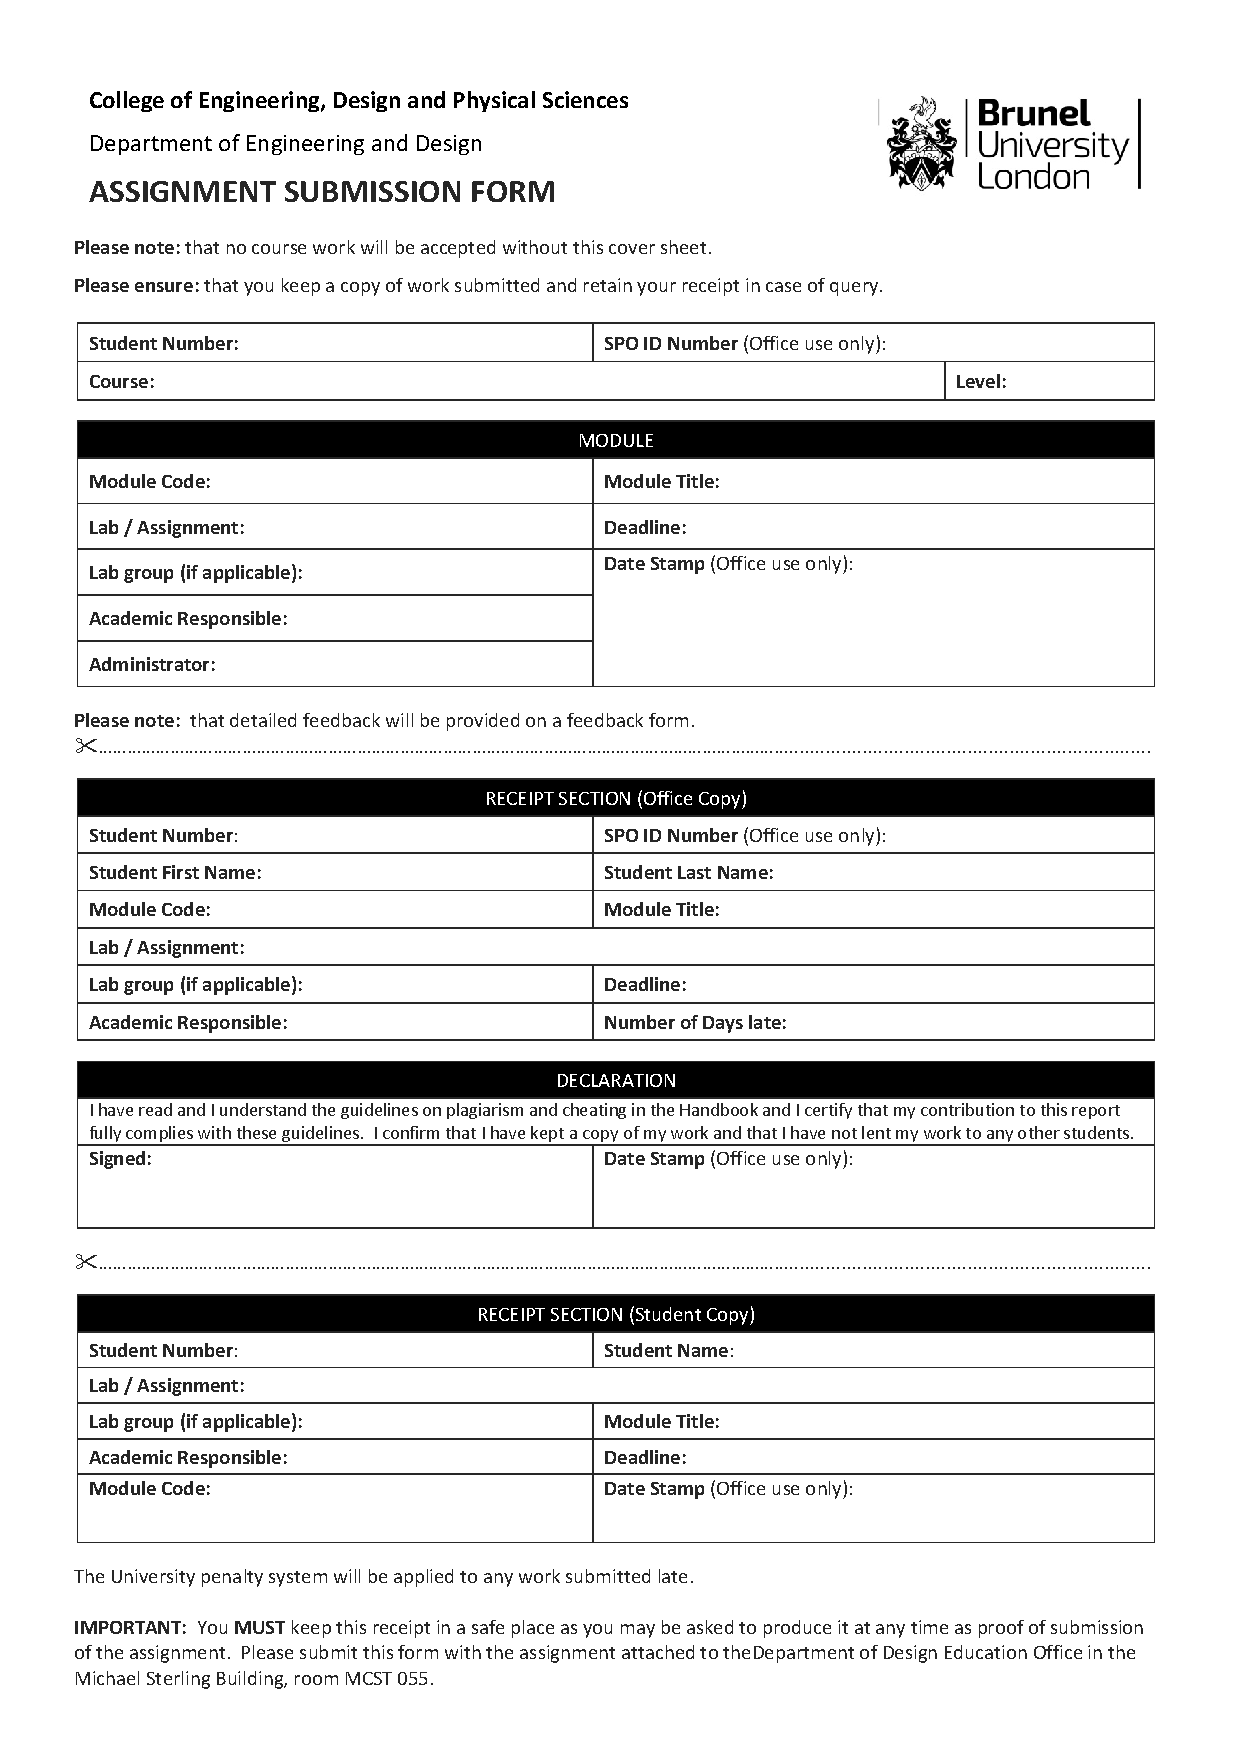
\includepdf{submission.pdf}
	\ofoot{\pagemark}

%	\listoftodos %Liste der todo-Marker
	
	%Danksagung
%	 \chapter*{Danksagung}
 \thispagestyle{empty} 
%\addcontentsline{toc}{chapter}{Danksagungen}

....Ich danke mir selbst f�r diese tolle Arbeit....
	
	%Quote
%	\pagenumbering{gobble}
\thispagestyle{empty}
\vspace*{\fill}
\epigraph%
{\glqq Ich habe hierf�r einen wahrhaft wunderbaren Beweis, doch ist dieser Rand hier zu schmal, um ihn zu fassen.\grqq}%
{\footnotesize\textsc{Pierre de Fermat}, 1637\textsuperscript{} - Randnotiz, die Generationen von Mathematikern besch�ftigte}
\vfill
\clearpage

% Seitennummerierung -----------------------------------------------------------
%   Vor dem Hauptteil werden die Seiten in gro�en r�mischen Ziffern 
%   nummeriert.
% ------------------------------------------------------------------------
	\pagenumbering{Roman}
	

	
 % Inhaltsverzeichnis --------------------------------------------------------	
	\tableofcontents

% Abk�rzungsverzeichnis --------------------------------------------------------
% f�r korrekte �berschrift in der Kopfzeile
%	%make index befehl zur erneuerung der Liste :

%makeindex Projekt-Industriemathematik.nlo -s nomencl.ist -o Projekt-Industriemathematik.nls

	\nomenclature{$x_t$}{Pose des Roboters zum Zeitpunkt $t$}%
	\nomenclature{$u_t$}{Ausgef�hrter Steuerbefehl zum Zeitpunkt $t$}%
	\nomenclature{$z_t$}{Erzeugte Messung zum Zeitpunkt $t$}%
	\nomenclature{$m$}{Erzeugte Karte der Umgebung}%
	\nomenclature{$x$}{x-Koordinate des Roboters}%
	\nomenclature{$y$}{y-Koordinate des Roboters}%
	\nomenclature{$\theta$}{Orientierung des Roboters}%
	\nomenclature{$v$}{Tangentiale Geschwindigkeit}%
	\nomenclature{$w$}{Rotationsgeschwindigkeit}%





	
%	\clearpage\markboth{\nomname}{\nomname} 
%	\printnomenclature
%	\label{sec:Symbole}

%Glossareintr�ge die nicht im Flie�text genutzt wurden auch Einbinden	
%	\glsaddall
	
%	%Befehl zur erzeugung von eine Glossar
%makeindex -l -s Bachelor-Thesis.ist -o Bachelor-Thesis.gls Bachelor-Thesis.glo


%make index befehl zur erneuerung der Liste :
%makeindex Bachelor-Thesis.nlo -s nomencl.ist -o Bachelor-Thesis.nls


	\newglossaryentry{SLAMGL}{%
	name=SLAM:,
	description={Simultane Lokalisierung und Kartierung (engl. simultaneous localization and mapping).},
	short = {SLAM},
	text = {Simultane Lokalisierung und Kartierung}
	}

	\newglossaryentry{Posen}
	{
	  name={Pose:},
	  description= {Als Pose oder r�umliche Lage wird im technischen Zusammenhang die Kombination von Position und Orientierung eines Objektes zu einem Zeitpunkt $t$ bezeichnet.},
	  text={\text{Pose}}
	}

	\newglossaryentry{Karte}{%
	name=Karte:,
	description={Enth�lt Informationen �ber die Umgebung, wie Position von Objekten/W�nden und stellt diese grafisch dar.}
	}

%	\clearpage\markboth{\nomname}{Glossar}
%	\label{sec:Glossars} 
%	\glossarystyle{indexgroup}
%	\printglossaries

	
% Tabellenverzeichnis--------------------------------------------------------
%	\listoftables 
	%\renewcommand{\lstlistlistingname}{Verzeichnis der Listings}
	%\lstlistoflistings % Listings-Verzeichnis
%	\listoffigures % Abbildungsverzeichnis

% arabische Seitenzahlen im Hauptteil ------------------------------------------
	\clearpage
	\pagenumbering{arabic}

% die Inhaltskapitel werden in "Inhalt.tex" inkludiert -------------------------
	             % Hier k�nnen die einzelnen Kapitel inkludiert werden. Sie m�ssen in den 
% entsprechenden .TEX-Dateien vorliegen. Die Dateinamen k�nnen nat�rlich 
% angepasst werden.


  % % % % Einleitung % % % % %
%	 \chapter{Einleitung und Motivation}
\label{einleitung-und-motivation}
Die Anforderungsanalyse ist mitunter das wichtigste Gebiet bei der Entstehung eines Systems. Die Literatur verwendet hierf�r den englischen Begriff des Requirements Engineering, der in dieser Arbeit weiter verwendet wird. Hierbei handelt es sich um die Qualit�tsanalyse von Anforderungen, die an ein System gestellt werden. Requirements (oder Anforderungen) sind die Kriterien, die ein System erf�llen muss. Dabei kann es sich sowohl um Software als auch um Hardware handeln.\\
Bisweilen wird sich auf die Erfahrung der Stakeholder\footnote{Engl. w�rtlich: Interessenvertreter, Anspruchsberechtigter, Projektbeteiligter} verlassen, um die Qualit�t der Anforderungsdokumente zu bestimmen. Dass dies in den meisten F�llen nicht ausreicht, zeigen folgende Statistiken.\\
Laut dem Chaos-Report von 2014 der Standish Group, werden 31.1\% der IT-Projekte vor der Fertigstellung abgebrochen \cite[vgl.][]{Gro14}. In Abbildung \ref{erfolgsraten} wird veranschaulicht, dass nur 16\% aller Projekte erfolgreich abgeschlossen werden. Gemeint ist, dass am Ende eines Projekts, keine Mehrkosten durch Verz�gerungen, Systemprobleme etc. verursacht worden sind. 
Des Weiteren wird behauptet, dass 52.7\% aller Projekte ca. 198\% teurer werden als eingeplant \cite[vgl.][]{Gro14}. Grund daf�r sind zum gr��ten Teil nicht korrekte Anforderungen (Kap. \ref{requirement-engineering}).
\begin{figure}[!htb]
	\centering
	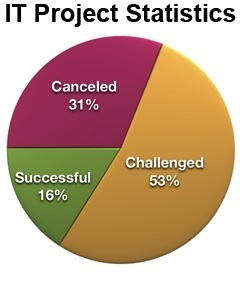
\includegraphics[width =0.4\textwidth]{ITProjectStatistics.jpg}
	\caption[IT-Projekt Erfolgsraten]{IT-Projekt Erfolgsraten \cite[vgl.][]{Gro14}}
	\label{erfolgsraten}
\end{figure}
\pagebreak
\begin{quote}
	\glqq Stolze 43 Prozent der im Betrieb festgestellten Fehler in Steuerungs- und Regelungssoftware sind Unzul�nglichkeiten in der Analysephase oder der Systemspezifikation zur�ckzuf�hren. 'Sie wirken sich viel sp�ter aus und kosten eine Menge Geld, wenn man sie beheben will.'\grqq~\cite{Zei14}
\end{quote}
Die Statistiken der Standish Group, sowie die Erkenntnisse aus \cite{Zei14} zeigen, dass selbst gro�e Unternehmen Schwierigkeiten haben korrekte Anforderungen zu formulieren, was die Wichtigkeit der Disziplin weiter unterstreicht. Je fr�her Unzul�nglichkeiten und Fehler in der Planung erkannt werden, desto einfacher und kosteng�nstiger sind diese zu beheben. Qualitativ hochwertige und pr�zise Anforderungen sind dabei der Schl�ssel zum Erfolg.\\
Aus diesem Grund w�re es ideal, wenn die Qualit�tspr�fung der Anforderungen im Requirements Engineering automatisiert ablaufen w�rde. Ein Tool, das auf Knopfdruck erkennt, ob die von den Stakeholdern gestellten Kriterien (Kap. \ref{qualit�tskriterien}) an eine Anforderung erf�llt sind, w�re erstrebenswert. Dieses Programm k�nnte in erheblich schnellerer Zeit als bisher m�glich, Anforderungen auf ihre Qualit�t �berpr�fen, ohne menschlichen Fehleinsch�tzungen unterworfen zu sein.

	\section{Aufgabenstellung und Kontext}
	\label{aufgabenstellung}
	Die Bachelorarbeit von Sebastian Zieschang \cite{Zie16}, sowie die Vorliegende, besch�ftigen sich mit den ersten Ans�tzen, wie ein entsprechendes Tool aufgebaut sein k�nnte, welche Algorithmen es verwenden sollte und welche computerlinguistischen Verfahren daf�r notwendig sind. Diese Arbeit besch�ftigt sich vorwiegend mit dem mathematischen Aspekt des Problems. Das hei�t, welche Algorithmen kommen in Frage, wie sind diese aufgebaut und wie sehen die Evaluierungsergebnisse des Experiments (siehe Kapitel \ref{daten-und-pipeline}) aus. Die Arbeit von Herr Zieschang geht weitestgehend auf die Computerlinguistik der Problemstellung ein.\\
	Als Ziel ist gesetzt, dass beide Bachelorarbeiten zusammen ein einfaches Tool zur ersten automatisierten Qualit�tsanalyse hervorbringen. Damit wird ein Grundstein f�r weitere Forschung auf diesem Themengebiet gelegt.\\
	Obwohl die manuelle Pr�fung der Anforderungen auf Qualit�t ein gro�er Aufwand ist, gibt es bis dato keine Bem�hungen dies zu automatisieren. Es wird lediglich gepr�ft ob Quellcodes den Anforderungen gen�gen \cite[vgl.][]{Wit+08}, nach Gemeinsamkeiten zwischen Anforderungen gesucht \cite[vgl.][]{Cyr+07} oder es werden weltweite Projekte mit dem \textit{verteilten Requirements Engineering} \cite[vgl.][]{HJL07} abgestimmt.\\
	Allein \cite{Rup00} und \cite{Rup07} legten den Grundstein zur nat�rlichsprachigen Qualit�tspr�fung von Anforderungen. Dieser zielt jedoch nicht auf die automatisierte Pr�fung ab, sondern beschr�nkt sich auf die sprachliche Theorie.\\
	Erstellt werden beide Bachelorarbeiten bei der Firma IT-Designers GmbH, welche als Dienstleister f�r verschiedene Unternehmen t�tig ist. S�mtliche Anforderungsdokumente, die zur Analyse herangezogen worden sind, stammen aus dem Automotiv-Bereich. 
	
	\section{Aufbau des Projekts}
	\label{aufbau}
	Das erste Kapitel des Projekts erkl�rt die Grundlagen des Requirements Engineering. Es wird ein allgemeiner Einblick in diese Disziplin gegeben, wobei Fehlerursachen und L�sungsm�glichkeiten diskutiert werden.\\
	Im zweiten Kapitel wird der Begriff des Textmining eingef�hrt, das eine Disziplin des Datamining ist. Zus�tzlich wird gezeigt in welchem Teilgebiet des Textmining sich die Problemstellung der Qualit�tsanalyse von Anforderungen bewegt.\\
	Das darauf folgende Kapitel erl�utert die Algorithmen und l�sst einen Einblick auf die dahinter stehende Mathematik zu.\\
	Das vierte Kapitel erkl�rt den Begriff eines Experiments, zeigt dessen Aufbau und liefert Informationen �ber die verwendeten Daten sowie �ber das Preprocessing.\\
	Die genutzten Methoden zur Evaluierung der Ergebnisse werden im f�nften Kapitel aufgef�hrt. Dieses stellt anschlie�end die Ergebnisse dieser Arbeit vor.\\
	Im letzten Kapitel werden alle wesentlichen Inhalte des Projekts zusammengefasst. Weiterhin wird ein Ausblick auf m�gliche zuk�nftige Forschung auf diesem Themengebiet aufgezeigt.
% 
 % % % Grundlagen % % % % % % % 
%	\addtocontents{toc}{\protect\newpage}
%	 \chapter{Requirements Engineering}
\label{requirement-engineering}
Wie bereits in der Einleitung erw�hnt, ist Requirements Engineering ein wichtiges Teilgebiet des Systementwicklungsprozesses.
Anforderungen bestimmen die Eigenschaften, die ein System erf�llen soll. Somit ist es f�r jedes Projekt von Beginn an unerl�sslich, die richtigen Anforderungen zu bestimmen, damit nicht �ber das Ziel hinaus bzw. in eine falsche Richtung entwickelt wird. In beiden F�llen endet dies in vermehrten Kosten und schadet der Zufriedenheit des Kunden.\\
In diesem Kapitel wird der Begriff des Requirements Engineering erkl�rt. Es wird erl�utert, was die Kriterien von qualitativ hochwertige Anforderungen sind, um im sp�teren Verlauf der Entwicklung m�glichst wenige Fehler zuzulassen. Es wird darauf eingegangen, wieso die Kriterien so wichtig sind und wie qualitativ schlechte Anforderungen entstehen. Diese sind mangelhaft formuliert und f�hren somit zu sp�teren Problemen w�hrend oder sogar nach der Entwicklung. Unter Zuhilfenahme von Satzschablonen wird im Detail gezeigt, wie eine optimale Satzstruktur von Anforderungen aussehen soll. Des Weiteren werden die beiden Arten von Anforderungen, sowie die empfohlene Formulierung einer qualitativ hochwertigen Anforderung erl�utert. Am Ende des Kapitels wird sich mit der rechtlichen Verbindlichkeit einer korrekt formulierten Anforderung besch�ftigt.
 
			\section{Wichtigkeit des Requirements Engineering}
			\label{wichtigkeit}
			\begin{quote}
				\glqq Eine recht naive und gef�hrliche Annahme versteckt sich au�erdem in der Zuversicht, dass Entwickler und Anwender es schon rechtzeitig merken werden, wenn Missverst�ndnisse auftreten, und diese durch Nachfragen leicht beseitigen k�nnen. Vielmehr ist es die Regel, dass Verst�ndnisl�cken auf beiden Seiten viel zu sp�t und manchmal gar nicht aufgekl�rt werden, so dass f�r den Anwender Unn�tzes mit viel M�he implementiert wird, und zugleich zentrale, aber bislang implizit gebliebene Anforderungen gerade noch nicht erf�llt sind.\grqq~\cite{FK+00}
			\end{quote}
			
			Wie bereits Christian Dahme in \cite{FK+00} feststellte, ist das fr�hzeitige Erkennen von Fehlern und L�cken in Anforderungen Voraussetzung f�r ein erfolgreiches Projekt. Dass ein fr�hzeitiges und konsequentes Requirements Engineering, bei wachsender Komplexit�t und Gr��e der heutigen Systeme, immer essentieller wird, zeigt folgendes Beispiel:\\
			Bei dem \textbf{Denver-Koffer-Debakel} sollte am Flughafen von Denver ein automatisches Gep�cksystem eingef�hrt werden. Durch eine zu geringe Fehlertoleranz des Systems, verl�ngerte sich die Entwicklung um 16 Monate. Dies hat zu einem Verlust von 3,25 Milliarden Dollar gef�hrt \cite[vgl.][]{Rup07}.\\ 
			Die wahrscheinlichste Ursache f�r dieses Problem sind qualitativ schlechte Anforderungen. Beispielsweise k�nnte die Fehlertoleranz nur ungenau angegeben worden sein oder die Anforderungen waren unvollst�ndig, da bestimmtes Wissen, bez�glich der Toleranz, vorausgesetzt wurde. Weitere m�gliche Fehlerquellen sind im folgenden Abschnitt aufgelistet.
			
			\section{Ursachen f�r qualitativ schlechte Anforderungen}
			\label{ursachen}
			Unter mangelnder Qualit�t von Anforderungen wird verstanden, dass die Anforderungsdokumente nicht die Kriterien erf�llen, um ein gew�nschtes System zu realisieren. Die Ursachen f�r die mangelnde Qualit�t von Anforderungen lassen sich auf folgende Punkte zur�ckf�hren \cite[vgl.][]{Rup07}:
			\begin{itemize}
				\item \textbf{Unklar formulierte Anforderungen}\\
				Dadurch werden Anforderungen interpretierbar oder sind nicht richtig durchdacht, d.h. es wird etwas gefordert, was sp�ter nicht oder zumindest nicht in der geforderten Variante ben�tigt wird.
				\item \textbf{Fehlende Anforderungen}\\
				F�hren zu einem unvollst�ndigen System.
				\item \textbf{Unvollst�ndige Anforderungen durch implizites Wissen}\\
				K�nnen zu einem nicht fertigen System f�hren und lassen Raum f�r Interpretationen.
				\item \textbf{Unterschiedliche Ebenen der Kommunikation}\\
				In Folge von Missverst�ndnissen innerhalb der Erstellung des Anforderungsdokuments und verschiedener Vorstellungen des Endprodukts kann es zu komplett unterschiedlichen Systemen kommen. Dies kann in manchen F�llen auch auf kulturelle Differenzen zur�ckzuf�hren sein.
			\end{itemize}
			Aus diesen Gr�nden ist es sinnvoll Qualit�tsmerkmale an die Anforderungen zu stellen, um �berfl�ssige Fehlerquellen zu minimieren. Der folgende Abschnitt zeigt die wichtigsten Kriterien auf und beleuchtet diese.
			
			\section{Kriterien und Merkmale von Anforderungen}
			\label{qualit�tskriterien}
			Es ist erstrebenswert, dass nicht jedes Unternehmen ihre eigenen Kriterien an die Anforderungen stellt. Diese w�rden komplett unterschiedlich ausfallen und somit w�rde es keinen gemeinsamen Nenner geben. Deswegen wurden verschiedene Standards ausgearbeitet, die eine uniforme Grundlage bilden. Die folgenden Qualit�tskriterien entsprechen dem 'IEEE Recommended Practice for Software Requirements Specifications' \cite{ICS98}.
			\begin{itemize}
				\item \textbf{Eindeutigkeit}\\
				Die Anforderung sollte von allen betroffenen Personen gleich verstanden werden. Es d�rfen keine verschiedene Interpretationen entstehen.
				\item \textbf{Modifizierbarkeit}\\
				\glqq �nderungen an den Anforderungen k�nnen einfach, vollst�ndig und konsistent unter Beibehaltung der vorhandenen Struktur und des verwendeten Stils durchgef�hrt werden\grqq~\cite{Bal09}.
				\item \textbf{Vollst�ndigkeit}\\
				Eine Anforderung muss eine Funktionalit�t vollst�ndig definieren.
				\item \textbf{Verfolgbarkeit}\\
				Jede Anforderung muss eine eindeutige Identifikationsnummer erhalten. Hierzu z�hlt auch die Versionierung der �nderungen und damit die Nachvollziehbarkeit der Aktualit�t.
				\item \textbf{Korrektheit}\\
				Die Anforderung ist korrekt, wenn das System sie erf�llen soll.
				\item \textbf{Konsistenz}\\
				Die Anforderung muss in sich widerspruchslos sein.
				\item \textbf{Pr�fbarkeit}\\
				Die Realisierung der Anforderung muss testbar sein.
			\end{itemize}
			Diese Punkte reichen aus, um Anforderungen zu erstellen, deren Qualit�t nicht als mangelnd beschrieben werden kann. F�r qualitativ hochwertige Dokumente wurden zus�tzliche Merkmale definiert. Diese sind keine Pflicht, helfen jedoch erheblich dabei die Anforderungen zu verbessern.
			\begin{itemize}
				\item \textbf{Abgestimmt}\\
				Alle beteiligten Personen sollen mit den Anforderungen einverstanden sein.
				\item \textbf{G�ltig und Aktuell}\\
				Die beschriebenen Funktionalit�ten sollen nicht veraltet sein.
				\item \textbf{Atomar}\\
				Eine Anforderung soll nur aus einem Satz bestehen.
				\item \textbf{Verst�ndlich}\\
				Es ist wichtig, die Anforderungen klar und verst�ndlich zu formulieren. Zum Beispiel hilft das Weglassen unn�tiger Fachbegriffe, um die Verst�ndlichkeit beizubehalten.
			\end{itemize}
				Wird sich strikt an diese Kriterien und Merkmale gehalten, k�nnen Anforderungen von hoher Qualit�t, ohne gr��eren Aufwand, erstellt werden.\\
				Ungeachtet dessen, ist es wichtig auf die Formulierung der S�tze und deren Struktur zu achten. Folgend wird auf diese Thematik eingegangen.
			
			\section{Satzstruktur und Formulierung}
			\label{satzstruktur}
			Meistens entstehen Fehler in den Anforderungen durch unpr�zise Formulierungen oder S�tze, die zu viel Raum f�r Interpretationen lassen. Deswegen wurden einige Regeln eingef�hrt, um diesen Missst�nden vorzubeugen.
			\begin{itemize}
				\item \textbf{Anforderungen sollen in vollst�ndigen S�tzen beschrieben werden.}\\
				Stichpunktartige S�tze sind zu unpr�zise und k�nnen zu Missverst�ndnissen f�hren.
				\item \textbf{Anforderungen sollen m�glichst kurz und pr�gnant gefasst sein.}\\
				Unn�tige Formulierungen sind zu vermeiden.
				\item \textbf{Je Anforderung darf nur ein Satz formuliert werden.}\\
				Dadurch wird die �bersichtlichkeit gef�rdert.
				\item \textbf{Verschachtelungen und Nebens�tze sind zu vermeiden.}\\
				Infolgedessen sind die Anforderungen einfacher zu verstehen und zu lesen. Manche Prozesse setzten jedoch gewisse Bedingungen voraus, um ausgef�hrt werden zu k�nnen. Solche Bedingungen m�ssen in einem vorausgehenden Nebensatz aufgef�hrt sein.
				\item \textbf{Und- und Oder-Verkn�pfungen m�ssen in einzelne S�tze aufgel�st werden.}\\
				Hierdurch wird die Eindeutigkeit der Anforderungen beg�nstigt.
				\item \textbf{Aufz�hlungszeichen sollen m�glichst vermieden werden.}\\
				In gleicher Weise sollen hier bevorzugt komplette, einzelne S�tze verfasst werden.
			\end{itemize}
			Anforderungsschablonen vereinfachen das Einhalten dieser Regeln.
			\begin{quote}
				\glqq Eine Anforderungsschablone ist ein Bauplan, der die syntaktische Struktur einer einzelnen Anforderung festlegt.\grqq~\cite{Rup07}
			\end{quote}
			Somit wird nur die Syntax der Anforderung vorgegeben, nicht ihre Semantik. Anlehnend an \cite{Rup07} folgen f�nf Schritte, die zeigen, wie eine qualitativ hochwertige Anforderungsschablone entsteht, die der komplexen deutschen Sprache gerecht wird:
			\begin{itemize}
				\item \textbf{Schritt 1 - Am Anfang steht der Prozess}\\
				Am Wichtigsten ist es, die Funktionalit�t des Systems zu definieren. Dies ist der sogenannte Prozess. Ein Prozess soll ausschlie�lich durch Verben dargestellt werden.
				\item \textbf{Schritt 2 - Charakterisieren der Aktivit�t des Systems}\\
				Je nachdem, ob es sich bei der Anforderung um eine selbst�ndige Aktivit�t handelt oder um eine Benutzerinteraktion, sind hier Schl�sselw�rter wie 'f�hrt ... aus' oder 'stellt ... zur Verf�gung' zu verwenden. Die Anforderungen sollen immer aktiv und positiv verfasst werden. Im Falle einer negativen Anforderung muss diese noch einmal hinterfragt werden z.B. ob diese n�tig ist.
				\item \textbf{Schritt 3 - Festlegen der rechtlichen Verbindlichkeit}\\
				In diesem Schritt soll die juristische Relevanz der Anforderung festgelegt werden (Kap. \ref{verbindlichkeit}).
				\item \textbf{Schritt 4 - Der Feinschliff}\\
				Vor das Prozesswort k�nnen eventuelle Erg�nzungen eingef�gt werden. Es ist wichtig, dass kein Raum f�r Interpretationen bleibt.
				\item \textbf{Schritt 5 - Formulierung von logischen und zeitlichen Bedingungen}\\
				In manchen F�llen sollen Funktionalit�ten nur zu bestimmten Zeitpunkten stattfinden. Es kann vorkommen, dass manche Prozesse andere voraussetzen oder zun�chst ein bestimmter Messwert erreicht werden muss, damit dieser sinnvolle Verwendung findet. Zu diesem Zeitpunkt k�nnen, falls n�tig, Bedingungen f�r die Anforderung eingef�gt werden. 
			\end{itemize}
			
			Die Abbildungen \ref{satzschablone} und \ref{satzschablone-bedingung} zeigen zwei Anforderungsschablonen der deutschen Sprache mit jeweils einer Beispielanforderung.
			\begin{figure}[!htb]
				\centering
				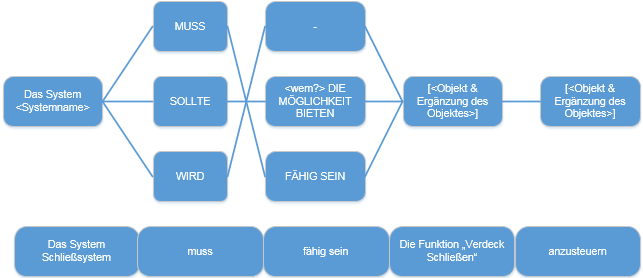
\includegraphics[width =1.0\textwidth]{satzschabloneVisio4.png}
				\caption[Deutsche Satzschablone ohne Bedingung]{Deutsche Satzschablone ohne Bedingung \cite[vgl.][]{Rup07}}
				\label{satzschablone}
			\end{figure}
			
			\begin{figure}[!htb]
				\centering
				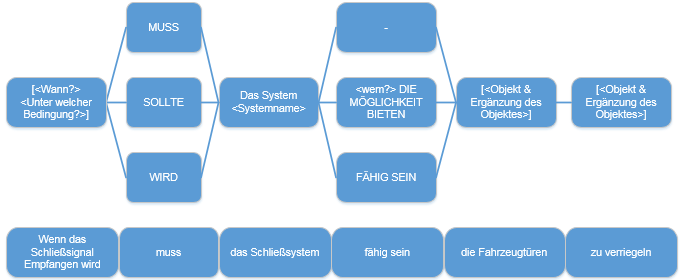
\includegraphics[width =1.0\textwidth]{satzschabloneBedingungVisio.png}
				\caption[Deutsche Satzschablone mit Bedingung]{Deutsche Satzschablone mit Bedingung \cite[vgl.][]{Rup07}}
				\label{satzschablone-bedingung}
			\end{figure}
			\pagebreak
			Ebenso wie die Qualit�tskriterien, entsprechen diese Satzschablonen dem 'IEEE 830-1998'-Standard. Mit ihnen ist es mit relativ geringem Aufwand m�glich Anforderungen zu erstellen, die musterg�ltig sind.\\
			Bisher wurde gezeigt, wie qualitativ hochwertige Anforderungen allgemein erstellt werden k�nnen. Es muss jedoch zwischen den verschiedenen Anforderungsarten unterschieden werden. In Abschnitt \ref{anforderungsarten} werden diese erl�utert.
			

			\section{Funktionale und nicht funktionale Anforderungen}
			\label{anforderungsarten}
			Im Allgemeinen wird zwischen den folgenden beiden Anforderungsarten unterschieden.\\
			\textbf{Funktionale Anforderungen} definieren eine vom System bereitzustellende Funktion. Hierzu z�hlen Verhaltensanforderungen, Strukturanforderungen und Funktionsanforderungen.
			\begin{quote}
				\textit{Das System soll f�hig sein, Walter finden zu k�nnen.}
			\end{quote}
			\textbf{Nicht funktionale Anforderungen} sind ein Oberbegriff f�r Qualit�tsanforderungen, wie z.B. Effizienz und Zuverl�ssigkeit. Beispiele w�ren technologische Vorgaben oder Hardware-Architekturen.
			\begin{quote}
				\textit{Das System muss Walter innerhalb einer halben Stunde gefunden haben.}
			\end{quote}
			Weiterhin k�nnen \textbf{Randbedingungen} von den Kunden vorgeschrieben werden, die eine dritte Art von Anforderungen bilden. Darunter fallen z.B. Termin zur Fertigstellung des Systems oder maximales Budget.\\
			Da unter den Stakeholdern (zwischen Kunde und Auftragsnehmer) immer ein rechtlicher Vertrag ausgehandelt wird, ist es unabdingbar der W�nsche der Kunden verbindlich in die Anforderungen einzuarbeiten. Nachstehend wird die rechtliche Verbindlichkeit der Anforderungsdokumente besprochen.
			
			\section{Rechtliche Verbindlichkeit}
			\label{verbindlichkeit}
			Jede Anforderung muss nach \cite{Rup07} eines der folgenden Modalverben\footnote{Verben die eine Notwenigkeit oder M�glichkeit zum Ausdruck bringen.} enthalten, die als Schl�sselw�rter dienen. F�r jedes dieser Verben besteht eine gewisse juristische Verbindlichkeit \cite[vgl.][]{Rup07}:
			\begin{itemize}
				\item \textbf{muss}\\
				Die darauf folgende Funktionalit�t ist zwingend zu erf�llen.
				\item \textbf{sollte}\\
				Die darauf folgende Funktionalit�t ist juristisch nicht verbindlich, zeigt jedoch Intentionen.
				\item \textbf{wird}\\
				Die darauf folgende Funktionalit�t deutet zuk�nftige Entwicklungen an, die ber�cksichtigt werden m�ssen.
			\end{itemize}
			Besitzt eine Anforderung keine dieser Schl�sselw�rter ist diese nicht annehmbar.\\
			F�r die Analyse der Anforderungsdokumente ist die Disziplin Textmining erforderlich. Daher besch�ftigt sich das n�chste Grundlagenkapitel mit diesem Thema.

\chapter{Textmining}
\label{textmining}
Wie bereits in Kapitel \ref{aufbau} angesprochen, werden Datamining und Textmining oft in Relation betrachtet. In der Disziplin Datamining wird das Ziel verfolgt, die Daten mithilfe von Algorithmen, nach Mustern zu durchsuchen, um die, f�r den entsprechenden Fall, n�tzlichen Informationen zu finden. Laut Ian H. Witten ist dabei die gr��te Herausforderung und die aufw�ndigste Arbeit, die vorhandenen Daten erst in das gew�nschte Ausgangsformat zu bringen und anschlie�end herauszufinden, wonach gesucht wird \cite[vgl.][]{WFH11}. Wo ist Walter? Ist das zu suchende Muster unbekannt, kann Walter kaum gefunden werden. Liegt jedoch die Information vor, dass er immer einen rot-wei� gestreiften Pullover, eine Brille und eine Pudelm�tze tr�gt, kann ihn ein Algorithmus ohne gr��eren Aufwand ausfindig machen.\\
Zusammengefasst geht es beim Datamining, um Techniken, die strukturelle Muster finden und beschreiben [vgl.][]\cite{WFH11}. Dieser Aufwand wird in Kauf genommen, damit m�glichst viele n�tzliche Informationen aus den vorhandenen Daten \glqq gesch�rft\grqq werden k�nnen.\\
Sollen Textdokumente klassifiziert oder nach Informationen  durchsucht werden, muss auf ein Teilgebiet des Datamining zur�ckgegriffen werden, dem Textmining. Mit Abbildung \ref{schnittstelle-text-data} wird deutlich, wie diese beiden Disziplinen zusammenh�ngen.
\begin{figure}[!htb]
	\centering
	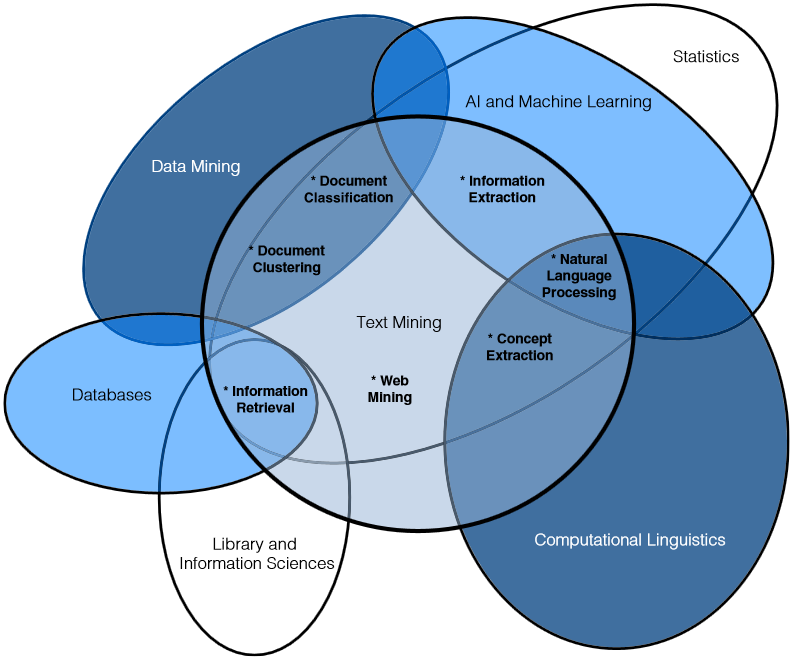
\includegraphics[width =0.75\textwidth]{SchnittstelleTextData.jpg}
	\caption[Schnittstellen des Textmining mit den sechs Teilgebieten]{Schnittstellen des Textmining mit den sechs Teilgebieten \cite[vgl.][]{Min+12}}
	\label{schnittstelle-text-data}
\end{figure}
An der Schnittstelle von Datamining und Textmining steht die Klassifikation von Dokumenten (Document Classification). Genau das entspricht der Qualit�tspr�fung von Anforderungen.
Der wesentlichste Unterschied zum Textmining ist der, dass beim Datamining, Muster in strukturierten Daten (z.B. Messwerte) gesucht werden. Textdokumente sind hingegen eine unstrukturierte Analysebasis. Lediglich aus der jeweiligen Grammatik der Sprache k�nnen Strukturen erkannt werden. Dieser Umstand macht es n�tig, die Disziplin der Computerlinguistik hinzuzuziehen, welche sich mit der computergesteuerten Verarbeitung menschlicher Sprache besch�ftigt. Der computerlinguistische Teil der Problemstellung der Qualit�tsanalyse von Anforderungsdokumenten ist nicht Gegenstand dieser Arbeit, weshalb hier nicht weiter darauf eingegangen wird. F�r interessierte Leser wird auf \cite{Car+10} verwiesen.\\
Abbildung \ref{prozess-textmining} zeigt die einzelnen Schritte im Prozess des Textmining. Diese Arbeit bewegt sich im Bereich der Textmining Methoden, sowie der Evaluation der Ergebnisse.
\begin{figure}[!htb]
	\centering
	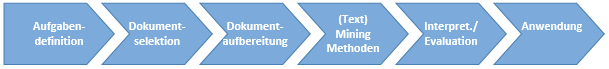
\includegraphics[width =0.9\textwidth]{textMiningProzessVisio.png}
	\caption[Der Prozess des Textmining]{Der Prozess des Textmining \cite[vgl.][]{HR06}}
	\label{prozess-textmining}
\end{figure}
		
		\section{Document Classification und dessen Algorithmen}
		\label{document-und-algorithmen}
		Sowohl im Datamining als auch im Textmining werden Algorithmen als Werkzeug genutzt. Sie basieren auf mathematischen und statistischen Grundlagen.\\
		Wie bereits erw�hnt (Kap. \ref{textmining}) entspricht die Qualit�tspr�fung von Anforderungsdokumenten dem Anwendungsgebiet der Document Classification. Hier geht es nicht um Informationsgewinnung, sondern darum, die Dokumente in Kategorien einzuteilen. Es ist zwischen bin�ren und multiplen Klassifikationen zu unterscheiden. Bei der bin�ren Klassifikation werden die Dokumente in zwei verschiedene Kategorien (z.B. Qualit�tspr�fung von Anforderungsdokumenten: gut, schlecht) unterteilt. Mehrere Kategorien hingegen, finden sich bei der multiplen Klassifikation. In der vorliegenden Bachelorarbeit wird sich ausschlie�lich auf bin�re Klassifikation der Anforderungen konzentriert. Diese werden in qualitativ minderwertige oder hochwertige Anforderungen klassifiziert. Mathematisch kann die Textklassifikation folgenderma�en definiert werden \cite[vgl.][]{MRS08}:
		
		\begin{minipage}{1\textwidth}
			\fbox{\parbox[c]{0.98\linewidth}{
					Sei $X$ die Menge der zu klassifizierenden Dokumente und $d \in X$ ein Dokument. Sei $C$ die Menge der Kategorien, in die $d$ klassifiziert werden kann und $c \in C$ eine Kategorie.
					Die Klassifikation ist eine Funktion $\phi$, die $d$ einer Klasse $c$ zuordnet:
					\begin{equation}
					\phi := X \rightarrow C
					\end{equation}
				}}
		\end{minipage}\\\\		
		Bei dem \textit{supervised Learning} (beaufsichtigtem Lernen) wird versucht, eine m�glichst gute Funktion $\phi$ aus der Menge $D$  abzuleiten.
		
			\begin{minipage}{1\textwidth}
				\fbox{\parbox[c]{0.98\linewidth}{
						Sei $D$ die Menge aller manuell klassifizierten Dokumente.
						\begin{equation}
							D = \{(d,c)|(d,c) \in X \times C\}
						\end{equation}
					}}
				\end{minipage}\\\\		
		Unter dem supervised Learning werden Lerntechniken verstanden, bei denen vordefinierte Kategorien auf Trainingss�tze gelegt werden \cite[vgl.][]{Kha+10}. Die Funktion $\phi$ wird automatisiert gesucht. Dabei helfen verschiedene Algorithmen. Im Gegensatz zum supervised Learning, gibt es noch die Lerntechniken des \textit{semi-supervised} und \textit{unsupervised} Learning. F�r interessierte Leser wird an dieser Stelle \cite{HS99} \cite{CSZ06} empfohlen. Diese Arbeit beschr�nkt sich auf das supervised Learning.\\
		Folgende Algorithmen sind laut \cite{Min+12} und \cite{WFH11} am besten f�r die Document Classification geeignet.
		\begin{itemize}
			\item \textbf{Na\"{i}ve Bayes}\\
			\vspace{-5mm}
			\item \textbf{Singular value decomposition (SVD)}\\
			\vspace{-5mm}
			\item \textbf{Logistic regression}\\
			\vspace{-5mm}
			\item \textbf{C4.5}\\
			\vspace{-5mm}
			\item \textbf{Neural network}\\
			\vspace{-5mm}
			\item \textbf{Support vector machines}\\
			\vspace{-5mm}
			\item \textbf{k-NN}\\
			\vspace{-5mm}
			\item \textbf{RIPPER}\\ 
		\end{itemize}
		Diese Algorithmen stammen aus dem Gebiet des maschinellen Lernens. Ian H. Witten beschreibt hier das Wort \textit{lernen} als Ver�nderung des Verhaltens durch k�nstliche Erfahrung auf eine Weise, die erlaubt zuk�nftig bessere Ergebnisse zu erzielen \cite[vgl.][]{WFH11}.
		
		\section{Ans�tze der Algorithmen}
		\label{ansaetze-der-algorithmen}
		Die im Kapitel \ref{document-und-algorithmen} aufgez�hlten Algorithmen verwenden unterschiedliche Ans�tze bei ihrem Vorgehen. Im Datamining werden sie in acht Kategorien eingestuft \cite[vgl.][]{WFH11}:
		\begin{itemize}
			\item \textbf{Ableiten rudiment�rer Regeln}\\
			Hier wird auf Grund eines Attributes entschieden, wie die Daten klassifiziert werden sollen. Dieses Vorgehen wird auch 1R (One-Rule) genannt.
			\item \textbf{Statistische Modelle}\\
			Im Gegensatz zu 1R werden bei diesen Modellen alle Attribute ber�cksichtigt. Es wird grundlegend davon ausgegangen, dass alle Attribute dasselbe Ma� an Bedeutung haben und unabh�ngig voneinander sind.
			\item \textbf{Divide et impera}\footnote{Divide and Conquer, Engl.: Teile und Herrsche}\\
			Bei diesem Vorgehen werden Entscheidungsb�ume erstellt. Es wird ein Attribut gew�hlt, welches als 'Root Node'\footnote{Engl.: Wurzelknoten, repr�sentiert die Wurzel eines Entscheidungsbaumes} dient. F�r jeden Wert dieses Attributes werden Zweige erstellt, an die weitere Knoten angeh�ngt werden, welche andere Attribute darstellen. Dies wird rekursiv fortgesetzt.
			\item \textbf{Covering\footnote{Engl.: Abdeckung, Bedeckung}-Algorithmen}\\
			Auch hier werden Entscheidungsb�ume erstellt. Es wird versucht, alle Daten in einen Bereich zu legen. Gleichzeitig werden alle Daten, die nicht in dieses Muster fallen, \glqq ausgesiebt\grqq. Diese werden mit dem gleichen Verfahren weiterhin ausgemustert.
			\item \textbf{Aufstellung von Verkn�pfungsregeln}\\
			F�r dieses Vorgehen m�ssen alle Kombinationen der vorhandenen Attribute erstellt werden. Da die Anzahl der Attribute oftmals sehr hoch ist, ist der Aufwand f�r die Erstellung meist unzumutbar.
			\item \textbf{Lineare Modelle}\\
			Bei den bisherigen Ans�tzen wurden nur nominale Attribute beachtet. Die linearen Modelle beziehen sich ausschlie�lich auf die numerischen Attribute. Das einfachste Beispiel w�re die Erstellung einer Regressionsgerade.
			\item \textbf{Instanzenbasiertes Lernen}\\
			Hier werden Trainingsdaten mit den zu klassifizierenden Daten verglichen, um den 'Nearest Neighbor'\footnote{Engl.: N�chster Nachbar} zu finden. Dieser wird zur Klasse der n�chsten Trainingsdaten gez�hlt.
			\item \textbf{Clustering}\\
			Das Clustering wird angewandt, wenn f�r die Daten bisher keine Klassen zur Einteilung vorhanden sind. Dieser Ansatz ist weitaus komplexer als die bisherigen.
		\end{itemize}
		Diese wissenschaftliche Arbeit wird sich nicht mit allen vorgestellten Algorithmen besch�ftigen, da es den vorgegebenen Rahmen �berschreiten w�rde. Welcher gew�hlte Algorithmus zu welchem Ansatz geh�rt, wird in Kapitel \ref{algorithmen} in der jeweiligen Ausf�hrung erw�hnt.

%
 % % % Hauptteil % % % % % % % %
	 
% Hauptkapitel
%
	\lstset{language=Java, numbers=left, numberstyle=\tiny, stepnumber=2, numbersep=5pt}
\chapter{Introduction}
\label{intro}
In today's world, where increasingly large amounts of data have to be processed and exchanged by distributed systems, the requirements for communication between distributed systems are becoming more and more complex. Not only performance is a problem, but also the requirement to make the services of the distributed systems available to several users at the same time. In other words, every system that is part of the architecture of a distributed system must be able to communicate with every other subsystem at the same time.\\
There are several technologies in the Java environment that can be used for communication within such a distributed system. The most basic variant is the use of Java Sockets. But this assignment favors the Java Remote Method Invocation. This report considers both technologies and presents a possible solution for a distributed system in which both of them play a role.
%%%%%%%%%%%%%%%%%%%%%%%%%%%%%%%%%%%%%%%%%%%%%%%%%%%%%%%%%%%%%%%%%%%%%%%%%%%%%%%%%%%%%%%%%%%%%%%%%%%%%%%%%
%%%%%%%%%%%%%%%%%%%%%%%%%%%%%%%%%%%%%%%%%%%%%%%%%%%%%%%%%%%%%%%%%%%%%%%%%%%%%%%%%%%%%%%%%%%%%%%%%%%%%%%%%
%%%%%%%%%%%%%%%%%%%%%%%%%%%%%%%%%%%%%%%%%%%%%%%%%%%%%%%%%%%%%%%%%%%%%%%%%%%%%%%%%%%%%%%%%%%%%%%%%%%%%%%%%
\chapter{Network Programming in Java}
\label{network-programming}
This chapter explains the theoretical basis for this assignment. The first section focuses on Java sockets, while the second deals with Remote Method Invocation (RMI). The aim is to highlight the differences as well as the advantages and disadvantages of both technologies.
\section{Sockets in Java}
A socket is an endpoint of a bi-directional communication connection between two programs running in different processes on the same computer or on different computers in a network . One socket takes on the role of the server, while the second socket acts as a client. Socket classes are used in Java to represent the connection between a client program and a server program. Sockets provide a simple API and require a hostname and a free port number to be initialized. If two or more sockets are running on the same computer, the hostnames and portnumbers must be different. Before the two processes (no matter if they are running on different computers or not) can communicate with each other, the client and server sockets must perform two different tasks.
\\
First of all, the client must know the hostname and port number of the server in order to connect to it. How exactly this is done depends on the programmer's decision. The server's address data can be stored permanently in the client's program code or can be retrieved by other techniques such as DNS. When establishing a connection between client and server, the client must also identify itself by sending its own host address to the server. The only thing the server has to do is to listen to possible clients attempting to open a connection.
\\
After the connection has been established, data can be transferred in both directions between server and client. The next two chapters show two different socket types and their differences.
\subsection{TCP Socket}
In general there are two different socket types. The first is the \textbf{Stream Socket} whose communication is based on the Transmission Control Protocol (\textbf{TCP}). Because TCP is connection oriented, the Three-Way-Handshake routine must be performed between server and client. This ensures a stable connection between the two end points via which data can be transmitted. TCP also has a built-in error recovery routine which automatically detects and attempts to fix connection terminations, lost data packets and other failures. The main advantage of this kind of socket is that the communication is safer, because lost packets are detected and resent by the sender (server or client). The main disadvantage is, that these sockets have a larger overhead with the complicated connection establishment and error recovery routines and are therefor slower. Figure \ref{tcpsocket} shows the necessary function calls, both Stream sockets must perform to establish a connection and transmit data:\\
\begin{figure}[H]
	\centering
	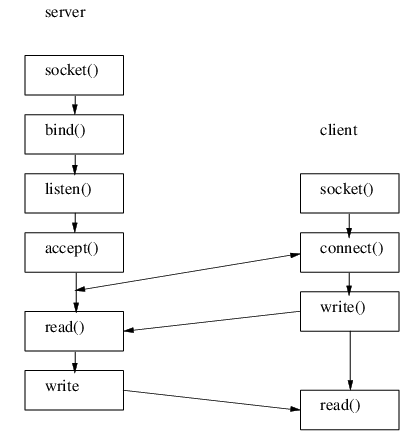
\includegraphics[width =0.7\textwidth]{tcpsocket.PNG}
	\caption{TCP communication between server and client}
	\label{tcpsocket}
\end{figure}
\subsection{UDP Socket}
The \textbf{Datagram Socket} is used for \textbf{UDP} (User Datagram Protocol) communication between two endpoints in the network or between two processes on the same computer.
\\Unlike TCP, UDP does not work connection-oriented. Here the transmitter sends its packets to the destination without worrying about whether the destination is reachable at all. There is also no error recovery because the sender doesn't care if its packets get lost or not. Datagram sockets are only used in certain use cases. Normally, the sender does care whether its packets arrive at their destination or not, which is why this type of communication is rarely used. UDP is only an alternative if the same information is repeated at short intervals, or if the receiver can easily restore missing information using the context. The main advantage however is that UDP is much faster than other network protocols. Figure \ref{udpsocket} shows the function calls both Datagram sockets must perform to transmit data to each other:\\
\begin{figure}[H]
	\centering
	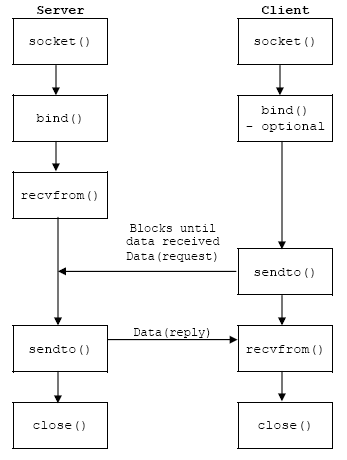
\includegraphics[width =0.6\textwidth]{udpsocket.PNG}
	\caption[Caption for LOF]{UDP communication between server and client\footnotemark}
	\label{udpsocket}
\end{figure}
\footnotetext{image-source: http:///www.tenouk.com//Module41a.html}
\section{Java Remote Method Invocation}
Remote Method Invocation (\textbf{RMI}) enables the call of a method of a remote Java object. The target object is located in another Java virtual machine that can run on a remote or local computer. The call looks exactly like a local call for the calling object, but special exceptions must be caught that can signal connection errors. This technique makes it very easy to build a distributed system in Java, which seems to communicate via normal method calls. For example, RMI can be used to outsource compute-intensive tasks to connected systems that have stronger processors or are simply less busy at the moment. 
\\
Again the basic architecture for RMI is distributed in a client and a server system. The server specifies an interface describing the method or methods that can be called remotely. This interface is called \textit{Remote Interface}. For the client to be able to call a remote method, it must also know this remote interface. The server however must provide a class which implements this interface and therefor provides a real method that can be invoked. This class must also inherit from the \textit{UnicastRemoteObject} class so that the JVM can create stubs and skeletons. The stub is a proxy object, which is required by the client to call the remote method. The skeleton is the proxy of the object on the server side.
\\
Because the remote method offers the possibility to pass parameters and return return values to the caller, some additional information has to be considered. It is possible to pass and return simply data types such as integers or strings without taking further action. But if the user wants to transfer complex objects such class-instances, their classes must implement the \textit{Serializable}-Interface.
\\
Parameters can be transferred via \textit{Object by Value} and \textit{Object by Reference}. The first means that a copy of the object is sent from the client to the server or the other way around. In the case of the second, a real reference to the object is transferred.
\\
The remote object (or service object) must be registered in the RMI registry, which is part of the JRMI environment. This is done with a unique name. This is necessary because the client uses this name to retrieve the object reference from this registry and thus obtains access to the service object. The communication between client and server is based on a simple request/reply protocol. This is why only the client can call methods on the server remotely. The other way around isn't possible. All server-methods that can be called remotely must also throw a \textit{RemoteException} if there is a connection error. Figure \ref{rmi} shows RMI's architecture:
\begin{figure}[H]
	\centering
	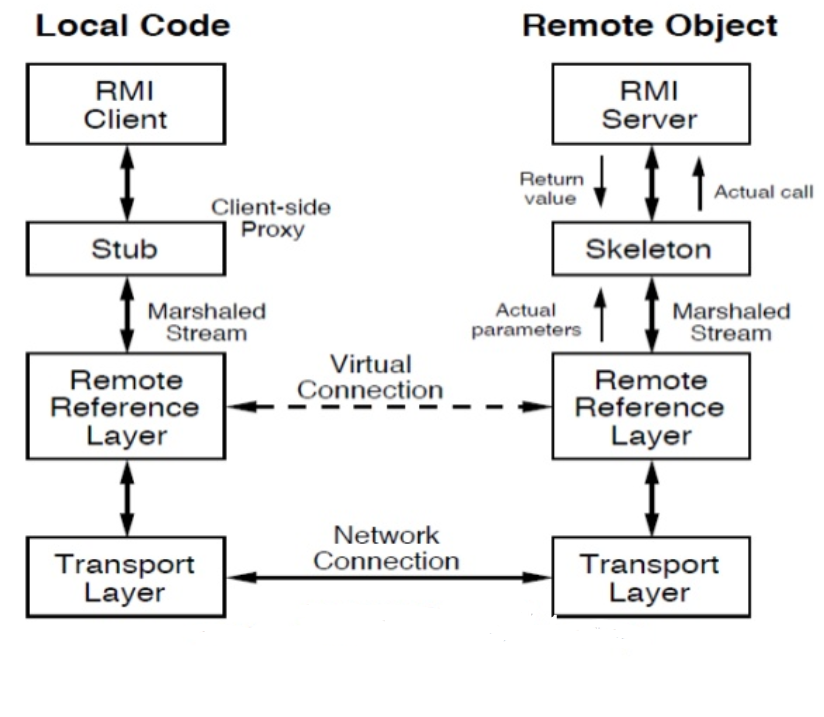
\includegraphics[width =0.8\textwidth]{rmi.png}
	\caption[Caption for LOF]{The RMI architecture\footnotemark}
	\label{rmi}
\end{figure}
\footnotetext{image-source: https://www.slideshare.net/tedionn/java-rmi-26537540}

%%%%%%%%%%%%%%%%%%%%%%%%%%%%%%%%%%%%%%%%%%%%%%%%%%%%%%%%%%%%%%%%%%%%%%%%%%%%%%%%%%%%%%%%%%%%%%%%%%%%%%%%%
%%%%%%%%%%%%%%%%%%%%%%%%%%%%%%%%%%%%%%%%%%%%%%%%%%%%%%%%%%%%%%%%%%%%%%%%%%%%%%%%%%%%%%%%%%%%%%%%%%%%%%%%%
%%%%%%%%%%%%%%%%%%%%%%%%%%%%%%%%%%%%%%%%%%%%%%%%%%%%%%%%%%%%%%%%%%%%%%%%%%%%%%%%%%%%%%%%%%%%%%%%%%%%%%%%%
\chapter{Job Server/Client Architecture}
\label{job}
\section{Overall Architecture}
\section{UDP-Multicast}
\section{The Job Server}
\section{The Job Client}
\section{Workload-Balancing}
%%%%%%%%%%%%%%%%%%%%%%%%%%%%%%%%%%%%%%%%%%%%%%%%%%%%%%%%%%%%%%%%%%%%%%%%%%%%%%%%%%%%%%%%%%%%%%%%%%%%%%%%%
%%%%%%%%%%%%%%%%%%%%%%%%%%%%%%%%%%%%%%%%%%%%%%%%%%%%%%%%%%%%%%%%%%%%%%%%%%%%%%%%%%%%%%%%%%%%%%%%%%%%%%%%%
%%%%%%%%%%%%%%%%%%%%%%%%%%%%%%%%%%%%%%%%%%%%%%%%%%%%%%%%%%%%%%%%%%%%%%%%%%%%%%%%%%%%%%%%%%%%%%%%%%%%%%%%%
\chapter{Other possible solutions}
\label{other-solutions}
\section{Server Broadcast}
\section{Workload Balancer}

%%%%%%%%%%%%%%%%%%%%%%%%%%%%%%%%%%%%%%%%%%%%%%%%%%%%%%%%%%%%%%%%%%%%%%%%%%%%%%%%%%%%%%%%%%%%%%%%%%%%%%%%%
%%%%%%%%%%%%%%%%%%%%%%%%%%%%%%%%%%%%%%%%%%%%%%%%%%%%%%%%%%%%%%%%%%%%%%%%%%%%%%%%%%%%%%%%%%%%%%%%%%%%%%%%%
%%%%%%%%%%%%%%%%%%%%%%%%%%%%%%%%%%%%%%%%%%%%%%%%%%%%%%%%%%%%%%%%%%%%%%%%%%%%%%%%%%%%%%%%%%%%%%%%%%%%%%%%%
\chapter{Conclusion}
\label{conclusion}

	
%	\chapter{Aufbau des Versuchs}
\label{daten-und-pipeline}
In diesem Kapitel werden die f�r die durchgef�hrten Versuche genutzten Daten vorgestellt (Kap. \ref{verwendete-daten}). Beim Datamining (sowie im Textmining, insbesondere der Textklassifikation) werden solche Versuche auch als Experimente bezeichnet \cite[vgl.][]{WFH11}, weswegen der Begriff des Experiments folgend verwendet wird. Weiterhin soll in diesem Teil der Arbeit, die n�tige Vorverarbeitung (Kap. \ref{vorverarbeitung}), die Erstellung der Attribute (Kap. \ref{features}) und die verwendete Pipeline (Kap. \ref{core}) erkl�rt werden. Zus�tzlich wird das genutzte Framework und der gebrauchte Lerner veranschaulicht.\\
F�r eine detailliertere Beschreibung der einzelnen Versuchskomponenten wird auf die Arbeit von Herr Zieschang \cite{Zie16} verwiesen.


	\section{Die verwendeten Daten}
	\label{verwendete-daten}
	Wie bereits in Kapitel \ref{aufgabenstellung} beschrieben, sind alle f�r das Experiment verwendeten Daten aus dem Bereich der Automobilentwicklung. Sie wurden im Rahmen der Bachelorarbeit von der Firma IT-Designers GmbH zur internen Verwendung zur Verf�gung gestellt. Somit handelt es sich um reale Anforderungsdokumente aus der Industrie und Praxis. Diese liegen im XML-Format vor. Ein Anforderungsdokument besteht nicht nur aus Anforderungen, sondern hat zus�tzlich erkl�rende Kommentare, Bilder, �berschriften und Kontaktdaten projektbetreuender Personen. Jeder Anforderung ist eine eindeutige ID zugewiesen.\\
	In der vorliegenden Form waren die Anforderungsdokumente nicht f�r das Experiment nutzbar. Wie diese f�r die Zwecke des Experiments bearbeitet worden sind, wird im n�chsten Abschnitt erl�utert.
	
	\section{Das Preprocessing}
	\label{vorverarbeitung}
	Die meisten der zur Verf�gung gestellten Daten, die f�r Experimente und Analyse verwendet werden sollen, liegen in einer Form vor, mit der nicht direkt gearbeitet werden kann. Dies liegt daran, dass die Daten mehr Informationen enthalten als ben�tigt. Das sind Informationen die f�r die spezifische Problemstellung irrelevant sind. Darunter fallen Kommentare, Bilder, �berschriften und Kontaktdaten. Solche Daten werden auch \textit{Noisy Data}\footnote{Engl.: verrauschte Daten} genannt und k�nnen die Ergebnisse von Experimenten massiv beeinflussen, was die Experimente nicht tragf�hig macht. Beispielsweise k�nnten weniger wichtige Attribute von den Algorithmen als wichtig erachtet werden, da diese h�ufig in den Noisy Data vorkommen. Werden diese vorher herausgefiltert, wird die H�ufigkeit dieses Attributes um einiges geringer. Somit sinkt die Relevanz des Attributes gleicherma�en.\\
	Aus diesem Grund ist das \textit{Preprocessing}\footnote{Engl.: Vorverarbeitung} notwendig. Bei dem Preprocessing werden die Daten auf einen einheitlichen Standard gebracht, welcher f�r die bevorstehenden Experimente ben�tigt wird. Die Daten werden gefiltert, damit sie m�glichst wenig irrelevante Informationen enthalten. Dabei muss beachtet werden, dass die Ursprungsdaten nicht zu sehr verf�lscht werden. Im Fall dieser Arbeit wurden Kommentare, Bilder, �berschriften und Kontaktdaten entfernt. Zumal die Art der Darstellung der Dokumente ebenso zum Preprocessing geh�rt \cite[vgl.][]{Kha+10}, wurden die ges�uberten Daten als Textdokumente gespeichert, um die weitere Verarbeitung zu vereinfachen. F�r das supervised Learning (Kapitel \ref{document-und-algorithmen}) sind bereits klassifizierte Daten erforderlich. Deswegen m�ssen die Anforderungen zuerst per Hand in die Klassen \textit{qualitativ hochwertig} und \textit{qualitativ minderwertig} zugeordnet werden.\\
	F�r die Experimente wird das Framework DKPro TC \cite{Dax+14} verwendet (siehe Kap. \ref{tc}). Das Framework verlangt, dass jede Anforderung in ein eigenes Textdokument geschrieben wird, da DKPro TC dies f�r die Inputdaten voraussetzt.\\
	
		\subsection{DKPro Core}
		\label{core}
		Da es sich bei den Anforderungen um nat�rlichsprachigen Text handelt, m�ssen die Anforderungen zus�tzlich mit diversen NLP\footnote{Abk.: Natural Language Processing, engl.: Verarbeitung nat�rlicher Sprache (Computerlinguistik)}-Werkzeugen vorbereitet werden, um nachfolgend Features (Kap. \ref{features}) darauf anwenden zu k�nnen. Gegenfalls muss eine Satzgrenzerkennung oder Tokenisierung durchgef�hrt werden. Ebenso k�nnen verschiedene Parser auf die Anforderungen angewandt werden.\\
		Da Programme, beziehungsweise Werkzeuge im Allgemeinen oftmals inkompatible In- und Outputs haben, ist es schwierig sie hintereinander zu verwenden, wie sie ben�tigt werden. Hierzu ist eine Pipeline\footnote{Engl.: Rohrleitung} notwendig, die die Formatprobleme zwischen den einzelnen Werkzeugen ausgleicht. DKPro Core\footnote{\url{https://www.ukp.tu-darmstadt.de/software/dkpro-core/}} bietet eine solche Pipeline \cite[vgl.][]{CG14}. Entwickelt wurde sie vom \textit{Ubiquitous Knowledge Processing Lab} der Universit�t Darmstadt. Diese Pipeline verbindet verschiedene NLP-Werkzeuge miteinander, die nach Bed�rfnis eingesetzt werden k�nnen.\\
		Mit Hilfe von DKPro Core k�nnen nun Features f�r die Anforderungen erstellt werden. Obwohl der Prozess der Definition von Features ebenfalls zu dem Preprocessing geh�rt \cite[vgl.][]{Kha+10}, wird dieser anschlie�end in einem separaten Unterkapitel beschrieben.\\
		
	
	\section{Die Features}
	\label{features}
	Im Gegensatz zu den Daten in Tabelle \ref{wetterdaten-numerisch}, sind die Attribute f�r Anforderungen nicht vorgegeben oder gar klar. Die Attribute mussten eigens f�r diese Arbeit erstellt werden. Dies geschieht mit Hilfe sogenannter Features. Meistens entspricht ein Feature einem Attribut. Es kann jedoch vorkommen, dass aus einem Feature mehrere Attribute generiert werden (vgl. N-Gram-Feature in der folgenden Aufz�hlung). Aufbauend auf den Erkenntnissen aus Kapitel \ref{requirement-engineering} folgt eine Aufz�hlung der ausgearbeiteten Features mit ihren Erkl�rungen.
	\begin{itemize}
		\item \textbf{Kleine Schablone}\\
		DKPro stellt einen Parser zur Verf�gung der f�r diese Arbeit genutzt worden ist. Es handelt sich dabei um den PCFG-Parser. Damit ist es m�glich einen Satz als Phrasenstrukturbaum darzustellen. Dabei wird der Satz in einzelne Phrasen zerlegt. Anhand dieser Phrasen ist es m�glich zu �berpr�fen ob der Aufbau der Anforderung den Schablonen aus Kapitel \ref{satzstruktur} entspricht. Bei diesem Feature soll auf die Schablone, die in Abbildung \ref{satzschablone} dargestellt wird, gepr�ft werden.
		\item \textbf{Gro�e Schablone}\\
		Wie beim vorherigem Feature soll hier ein Attribut durch Pr�fung des Attributes auf eine vorgegebene Schablone (Abbildung \ref{satzschablone-bedingung}) erstellt werden.
		\item \textbf{Tiefe des Satzes}\\
		Bei der Arbeit mit dem PCFG-Parser ist aufgefallen, dass er im Wesentlichen bei qualitativ schlechten Anforderungen tiefere B�ume aufbaut. Je verschachtelter ein Satz ist, desto tiefer wird der Baum. Wie in Kapitel \ref{qualit�tskriterien} und \ref{satzstruktur} diskutiert wurde, ist diese Eigenschaft bei Anforderungen nicht erw�nscht. Das erstellte Attribut aus diesem Feature gibt die numerische Tiefe des Satzes bzw. dessen Baumes an.
		\item \textbf{Anzahl der Phrasen}\\
		Ebenso mit Hilfe des Parsers, wurden die Phrasen einer Anforderung gez�hlt. Viele Phrasen bedeuten im Regelfall lange S�tze. Diese Eigenschaft deutet wiederum auf qualitativ schlechte Merkmale. Das erzeugte Attribut aus diesem Feature gibt die Anzahl der Phrasen einer Anforderung an.
		\item \textbf{Struktur}\\
		Dieses Feature �berpr�ft, �hnlich den Features \textit{Kleine Schablone} und \textit{Gro�e Schablone}, den Aufbau des Satzes. Beispielsweise wird gepr�ft ob ein Verb am Satzanfang steht. Bei qualitativ hochwertigen Anforderung steht das Verb meist im hinteren Teil des Satzes, da es sich dabei um den Prozess handelt. Am Anfang des Satzes w�re demnach ein Substantiv erw�nscht, da dieses das System beschreiben w�rde.
		\item \textbf{Bad Words}\\
		Dieses Feature erstellt ein Attribut, das die Anzahl der \textit{Bad Words} angibt. Im Rahmen dieser Bachelorarbeit wurden alle W�rter Bad Words genannt, die ein Indiz daf�r sind, dass es sich um eine qualitativ schlechte Anforderung handelt. Beispielweise W�rter die eine Negation aufzeigen (nicht, kein). In Kapitel \ref{requirement-engineering} wurde darauf eingegangen.
		\item \textbf{Konjunktionen}\\
		Dieses Feature ist dem Bad Words-Feature sehr �hnlich. Hier werden Konjunktionen in den Anforderungen gez�hlt. Diese Worte weisen auf Verbindungen zwischen S�tzen hin. In Kapitel \ref{satzstruktur} wurde gezeigt, dass dies bei Anforderungen nicht erw�nscht ist.
		\item \textbf{Count Tokens}\\
		Hier wurde die Anzahl der vorkommenden W�rter in einer Anforderung gez�hlt. Je mehr W�rter eine Anforderung hat, desto l�nger ist sie. Nach Kapitel \ref{satzstruktur} sollen Anforderungen m�glichst kurz gefasst werden.
		\item \textbf{Modalverb}\\
		Das mit am wichtigste an einer Anforderung ist das Modalverb. Dieses gibt die rechtliche Verbindlichkeit an (Kap. \ref{verbindlichkeit}). Existiert kein Modalverb in einer Anforderung, ist diese rechtlich nicht verbindlich. Hier wird ein Attribut erstellt das anzeigt ob ein Modalverb in der Anforderung vorhanden ist. Ist das nicht der Fall, kann direkt von einer qualitativ schlechten Anforderung ausgegangen werden.
		\item \textbf{Anzahl der Kommas}\\
		Hieraus wurde ein Attribut generiert, dass die Anzahl der Kommas in der Anforderung wiedergibt. Der Grund f�r dieses Attribut ist, dass in qualitativ guten Anforderungen maximal zwei bis drei Kommas vorkommen sollten. Eine h�here Anzahl von Kommas deutet auf einen verschachtelten Satz hin, was bei Anforderungen unerw�nscht ist (Kap. \ref{satzstruktur}).
		\item \textbf{Anzahl der S�tze}\\
		Wie aus Kapitel \ref{satzstruktur} hervorgeht, soll pro Anforderung nur ein Satz verwendet werden. Dieses Feature erstellt ein Attribut, dass die Anzahl der S�tze in den Anforderungen anzeigt.
		\item \textbf{Abh�ngigkeitstokens}\\
		F�r dieses Feature wurde ein \textit{Dependenz-Parser} verwendet. Mit einem Dependenz-Parser k�nnen Abh�ngigkeiten der W�rter eines Satzes ermittelt werden. Des Weiteren kann �berpr�ft werden um welche Art von Abh�ngigkeit es sich dabei handelt.
		\item \textbf{Bedeutung des Modalverbs}\\
		Wie bereits in Kapitel \ref{verbindlichkeit} erw�hnt, ist das Modalverb essentiell f�r eine Anforderung. Es kann jedoch vorkommen, dass ein Modalverb in einem Satz nicht als dieses verwendet wird, sondern als ein Hilfsverb im Satz steht. Als solches stellt das Modalverb keine rechtliche Verbindlichkeit sicher. Somit deutet dieser Fall auf eine qualitativ minderwertige Anforderung, es sei denn, es existiert ein weiteres Modalverb in dem Satz, dass auch wirklich als solches verwendet wird. Mit Hilfe des Dependenz-Parser kann dieser Umstand gepr�ft werden.
		\item \textbf{N-Gram}\\
		Aus diesem Feature werden $N$-viele Attribute generiert. Mit dem N-Gramm werden in diesem Fall die Anzahl der vorkommenden W�rter in den jeweiligen Klassen gez�hlt. Die daraus resultierenden Attribute geben die H�ufigkeit der $N$ h�ufigsten Wortes in einer Klasse an.
	\end{itemize}
		
	\section{Das Framework}
	\label{tc}
	Jedes Textmining-Experiment l�uft mit einem bestimmten Prozess ab, wie Abbildung \ref{prozess-textmining} zeigt. Vereinfacht, kann der Prozess auch wie folgt dargestellt werden.
		\begin{equation*}
			\text{Einlesen der Daten} \to \text{Preprocessing} \to \text{Trainieren} \to \text{Evaluation}
		\end{equation*}
	DKPro TC\footnote{https://www.ukp.tu-darmstadt.de/software/dkpro-text-classification/} ist ein Framework, das auf Text Classification ausgerichtet ist. Es erstellt �berwachte Lernexperimente, die nach obigem Muster aufgebaut werden \cite[vgl.][]{Dax+14}. Ein gro�er Vorteil liegt hier darin, dass sich das Framework um die Verkn�pfung der Textminingschritte k�mmert. Es muss nur darauf geachtet werden, dass die Inputdaten in gew�nschter Form vorliegen. In dem Fall von DKPro TC muss jede Anforderung in eine Textdatei geschrieben werden. Des Weiteren m�ssen die ben�tigten Features und ein Lerner angegeben werden, sowie die Algorithmen, welche vom Lerner bereit gestellt werden.\\
	Im n�chsten Abschnitt wird der verwendete Lerner beschrieben.
	
	\section{Der Lerner}
	\label{weka}
	Textklassifikationen k�nnen in zwei unterschiedliche Gruppen eingeteilt werden. Die eine ist das sogenannte \textit{Single Label Experiment}, wobei die andere \textit{Multi Label Experiment} genannt wird. Bei der ersteren kann ein Text nur einer Kategorie zugeordnet werden. Bei dem Multi Label Experiment kann er hingegen mehreren Kategorien zugeordnet werden. Ein gutes Beispiel f�r das Single Label Experiment ist ein Hund. Wird vorausgesetzt der Hund ist reinrassig, kann er entweder Labrador oder Mastiff sein. Beides gleichzeitig ist nicht m�glich. Die Artikel in der Online-Enzyklop�die Wikipedia\footnote{\url{https://www.wikipedia.org/}} sind hingegen meist in mehrere Kategorien eingeteilt. Der Artikel �ber den Vogel Wekaralle beispielsweise, ist in zwei Kategorien eingeteilt: \textit{Endemischer Vogel Neuseelands} und \textit{Rallenv�gel}.\\
	Obwohl das verwendete Framework DKProTC drei verschieden Lerner bereitstellt (WEKA\footnote{\url{http://www.cs.waikato.ac.nz/ml/weka/}}, MEKA\footnote{\url{http://meka.sourceforge.net/}}, Mallet\footnote{\url{http://mallet.cs.umass.edu/}}), sind nicht alle f�r den Rahmen dieser Bachelorarbeit geeignet. Beispielsweise ist MEKA ausschlie�lich f�r Multi Label Experimente gedacht. MALLET wiederum bietet eine eingeschr�nkte Auswahl an Algorithmen. Da es sich bei diesem Projekt um ein Single Label Experiment handelt und WEKA eine breite Auswahl an Algorithmen bietet wurde sich letztendlich f�r diesen entschieden.\\
	
%	\chapter{Training und Evaluation}
\label{training-und-evaluation}
In dem vorherigen Kapitel wurden die f�r die Versuche ben�tigten Hilfsmittel, sowie die verwendeten Daten beschrieben. In diesem Kapitel soll aufgezeigt werden, auf welche verschiedenen Arten sich ein Lerner trainieren l�sst. Des Weiteren werden zwei verschiedene M�glichkeiten erl�utert, die beschreiben, wie die Ergebnisse ausgewertet werden k�nnen. Folgend werden die einzelnen Experimente, chronologisch geordnet, aufgezeigt und evaluiert.
	
	\section{Trainingsmethoden}
	\label{trainingsmethoden}
	Um einen funktionierenden Klassifizierer zu erhalten, muss zuvor der Lerner trainiert werden. Das geschieht beim supervised Learning (Kap. \ref{document-und-algorithmen}) mit vorklassifizierten Datens�tzen. WEKA stellt dabei zwei verschiedene Methoden zur Verf�gung. Beide Methoden werden anschlie�end vorgestellt. Unabh�ngig von der Traningsmethode gilt: Je mehr Daten f�r das Training zur Verf�gung stehen, desto akkurater wird die Klassifikation.
	
		\subsection{Percentage Split}
		\label{split}
		Das wohl gel�ufigste Verfahren ist die des Aufteilens der vorhandenen Daten in zwei Teile. Ein Teil der Daten wird ausschlie�lich f�r das Training verwendet, wobei der andere nur zu Testzwecken existiert. Je gr��er der Anteil der f�r das Training zugeteilten Daten, desto bessere Ergebnisse k�nnen erwartet werden. Der Trainingsanteil sollte jedoch nicht zu hoch sein, da sonst zu wenig Daten f�r das Testen und Evaluieren vorhanden w�ren. Standardm��ig werden $66\%$ der Daten f�r das Training verwendet \cite[vgl.][]{WFH11}.\\
		Der, durch die Trainingsdaten, trainierte Lerner wird auf die Testdaten angewandt. Je nach Klassifikationsergebnis k�nnen die Features angepasst werden. Daraufhin wird nochmals mit den Trainingsdaten trainiert. Dieses Verfahren wird in WEKA als Percentage Split bezeichnet. Die Unterteilung der Daten ist n�tig, um den Lerner nicht nur an die Trainingsdaten anzupassen. Dieses Ph�nomen wird als Overfitting bezeichnet. Es k�nnen extrem gute Ergebnisse anhand der Daten, die f�r das Training verwendet worden sind, erzielt werden. F�r bis dahin unber�hrte Daten ist der so trainierte Klassifizierer hingegen nicht aussagekr�ftig.\\
		Oftmals werden die Daten nicht in zwei, sondern drei Teile geteilt \cite[vgl.][]{WFH11}. Hier werden die Datenteile als Trainingsdaten, Validationsdaten und Testdaten bezeichnet \cite[vgl.][]{WFH11}. Die Validationsdaten k�nnen aus mehreren Sets bestehen, was bedeutet, dass die Daten nicht in drei gleichgro�e Teile geteilt werden m�ssen.\\
		Das Vorgehen ist hierbei folgendes. Der Lerner bekommt die Trainingsdaten zum Trainieren. Anschlie�end wird auf einem Set der Validationsdaten getestet. An dieser Stelle k�nnen die Features je nach Bedarf angepasst werden. Das verwendete Set wird danach zu den Trainingsdaten hinzugef�gt und es wird erneut trainiert. Sind mehrere Sets von Validationsdaten vorhanden, kann dieser Vorgang �fters wiederholt werden. Anschlie�end wird auf den, bis dahin unber�hrten, Testdaten getestet.\\
		Geeignet ist dieses Trainingsverfahren, wenn eine gro�e Anzahl an Daten zur Verf�gung steht, da immer m�glichst viele Trainingsdaten f�r bestm�gliche Ergebnisse ben�tigt werden.
		
		\subsection{Cross-Validation}
		\label{cross-validation}
		Ist die Anzahl der Daten (und somit die Anzahl der m�glichen Trainingsdaten) gering oder begrenzt, ergibt sich das Problem, dass der Lerner nur ungen�gend trainiert werden kann. Daraus resultiert eine ungenaue Klassifikation.\\
		Bei der \textit{n-Fold Cross-Validation} werden die Daten in $n$ gleichgro�e Teile aufgeteilt. Ein Teil davon wird f�r den Test verwendet, w�hrend $n-1$ Teile f�r das Training zu Verf�gung stehen. Ist ein Trainings- und Testdurchlauf beendet, wird ein anderer Teil aus den $n$ Teilen f�r das Testen verwendet. Die restlichen Daten werden wie im Percentage Split als Trainingsdaten genutzt. Dieser Prozess wird so oft durchgef�hrt, bis mit allen Teilen einmal getestet worden ist. Ist das der Fall, ist ein n-Fold Cross-Validation Durchlauf beendet. Da die Daten zuf�llig in $n$ Teile geschnitten werden, ist es �blich die n-Fold Cross-Validation wiederholt durchzuf�hren. In \cite{WFH11} wird vorgeschlagen diese Wiederholung $n$-mal auszuf�hren. Der Standardwert f�r $n$ liegt laut \cite{WFH11} bei 10.\\
		Eine weitere M�glichkeit ist das \textit{Leave-One-Out Cross-Validation}. Bei dieser Methode werden die Daten in $n$ Teilst�cke unterteilt. Wobei hier $n$ die Anzahl der Objekte ist. Dabei wird an einem Objekt getestet und an dem Rest trainiert. Ein Durchlauf ist beendet, sobald an allen Objekten einmal getestet worden ist. Hierbei ist es nicht notwendig die Cross-Validation mehrere Male durchzuf�hren, da es in diesem Fall keinen zuf�lligen Schnitt gibt.\\
		Da f�r diese Bachelorarbeit keine vorklassifizierten Anforderungen vorhanden waren, mussten diese von Hand klassifiziert werden. Der dazugeh�rige Prozess ist so zeitaufwendig, dass er den Rahmen der Bachelorthesis gesprengt h�tte. Aufgrund dessen steht nur eine begrenzte Anzahl an Daten f�r dieses Projekt zur Verf�gung. Aus diesem Grund wurde mit dem n-Fold Cross-Validation ($n=10$) trainiert. F�r die Methode des Percentage Split w�ren mehr Daten n�tig gewesen.
	
	\section{Evaluationsmethoden}
	\label{evaluationsmethoden}
	In diesem Abschnitt werden zwei g�ngige Methoden vorgestellt, die f�r das Auswerten von Klassifikationsergebnissen verwendet werden. Die erste Methode nennt sich die ROC-Methode, die Zweite ist die sogenannte PR-Methode. Beide M�glichkeiten basieren auf der sogenannten \textit{Confusion Matrix}, welche nachfolgend erkl�rt wird.
	
		\subsection{Confusion Matrix und ihre Werte}
		Bei der bin�ren Klassifikation sind nur vier F�lle m�glich, in welche der Klassifikator die Objekte kategorisieren kann. Ausgehend von der Annahme, ein Objekt wird bewertet, ergeben sich folgende M�glichkeiten.
		\begin{itemize}
			\item \textbf{True Positive (tp)}\\
			Das Objekt wurde richtig klassifiziert. Das hei�t,  das Objekt geh�rt zur Klasse A und wurde als diese erkannt.
			\item \textbf{False Positive (fp)}\\
			Das Objekt wurde falsch klassifiziert. In diesem Fall wurde das Objekt als Element der Klasse A erkannt, obwohl es dies nicht ist.
			\item \textbf{True Negative (tn)}\\
			Das Objekt wurde richtig klassifiziert. Das Objekt geh�rt zur Klasse B und wurde auch als dieses erkannt.
			\item \textbf{False Negative (fn)}\\
			Das Objekt wurde falsch klassifiziert. Hier wurde das Objekt in Klasse B kategorisiert, obwohl es zur Klasse A geh�rt.
		\end{itemize}
		Aus diesen F�llen ergibt sich die Confusion Matrix. Dabei werden die H�ufigkeiten der auftretenden F�lle (tp, fp, tn, fn) in einer $2 \times 2$-Matrix dargestellt. Im Idealfall treten die F�lle False Negativ und False Positive nicht auf. Tabelle \ref{confusion-matrix} zeigt die Confusion Matrix, die sich f�r das Beispiel der Qualit�tsanalyse von Anforderungen ergibt.
		
		\begin{table}[!htb]
			\centering
			\begin{tabular}{|c|c|c|}
				\hline
				& Klasse A & Klasse B \\ \hline
				Klasse A   & Anzahlt  $tp$           & Anzahl $fn$               \\ \hline
				Klasse B & Anzahl $fp$            & Anzahl $tn$              \\ \hline
			\end{tabular}
			\vspace{3mm}
			\caption{Confusion Matrix im Fall der Qualit�tsanalyse von Anforderungen}
			\label{confusion-matrix}
		\end{table}
		Sowohl die ROC-Methode, als auch die PR-Methode basieren auf einer Confusion Matrix. Das n�chste Unterkapitel erl�utert die Idee der ROC-Methode.
	
		\subsection{ROC-Methode}
		Aus den Werten der Confusion Matrix k�nnen verschiedene Kenngr��en berechnet werden. Hier wird zwischen Sensitivit�t (auch Richig-Positiv-Rate oder Recall genannt), Falsch-Negativ-Rate, Spezifit�t (auch Richtig-Negativ-Rate genannt) und Falsch-Positiv-Rate (auch false alarm rate genannt) unterschieden. Mit diesen Werten kann gut erkannt werden, wie sich der Klassifizierer in bestimmten Situationen verh�lt.\\
		Die Sensitivit�t gibt in diesem Fall an, wie viel Prozent der Anforderungen der Klasse \textit{Qualitativ hochwertig}
		tats�chlich erkannt worden sind. Die Falsch-Negativ-Rate zeigt den Anteil der Objekte an, die f�lschlicherweise als qualitativ minderwertig deklariert worden sind. Die Spezifit�t und Falsch-Positiv-Rate geben die gegenteiligen Werte an. Das hei�t im Falle der Spezifit�t, dass sie anstatt die Anzahl der korrekt in \textit{Qualitativ hochwertig} klassifizierten Objekte, die Rate der korrekt in \textit{Qualitativ minderwertig} darstellt.
		
		\begin{minipage}{1\textwidth}
			\fbox{\parbox[c]{0.98\linewidth}{
					\begin{align}
					\text{Sensitivit�t} &= \frac{\text{Anzahl} ~tp}{\text{Anzahl} ~tp +\text{Anzahl}~fn}\\
					\text{Falsch-Positiv-Rate} &= \frac{\text{Anzahl} ~fp}{\text{Anzahl} ~fp +\text{Anzahl}~tn}\\
					\text{Spezifit�t} &= \frac{\text{Anzahl} ~tn}{\text{Anzahl} ~tn +\text{Anzahl}~fp}\\
					\text{Falsch-Negativ-Rate} &= \frac{\text{Anzahl} ~fn}{\text{Anzahl} ~fn +\text{Anzahl}~tp}
					\end{align}
				}}
		\end{minipage}\\\\
		Die \textbf{R}eceiver \textbf{O}perating \textbf{C}haracteristic-Methode (kurz ROC) verwendet zwei dieser Kenngr��en um eine Kurve zu zeichnen. Die Sensitivit�t wird auf der y-Achse abgebildet, die Falsch-Positiv-Rate auf der x-Achse \cite[vgl.][]{Faw06}. Die dabei entstehende Ebene wird ROC-Space genannt und hat einen Gesamtfl�cheninhalt von genau $1$, da der ROC-Space sowohl auf der x-Achse als auch auf der y-Achse bis zum Wert $1$ betrachtet wird. Dies entspricht einer Rate von $100\%$. Ist somit die Sensitivit�t $=1$, kommt das einer Trefferquote der qualitativ hochwertigen Anforderungen von $100\%$ gleich. Dies muss dennoch nicht bedeuten, dass der Klassifikator pr�zise arbeitet. Es k�nnte der Fall sein, dass er jedes Objekt schlicht als positiv kategorisiert. Somit w�ren alle Objekte, ob qualitativ hoch- oder minderwertig derselben Klasse zugeordnet. Deshalb wird der Fl�cheninhalt unter der so genannten ROC-Kurve betrachtet. \\
		Der Fl�cheninhalt, auch als ROC-AUC\footnote{Area under curve} bekannt, unter der Kurve zur x-Achse ist wie folgt interpretierbar. Ist dieser gleich dem Fl�cheninhalt der ersten Winkelhalbierenden ($y=x$), betr�gt er somit $0.5$, steht dies f�r einen Zufallsprozess des Klassifikatiors \cite[vgl.][]{Faw06}. Eine theoretische ROC-AUC von $1$, w�rde einer perfekten Klassifikation entsprechen \cite[vgl.][]{Faw06}. Liegt der Wert der ROC-AUC zwischen $0$ und $0.5$ spricht das f�r eine umgekehrte Klassifikation, das hei�t, die Objekte m�ssten jeweils der anderen Klasse zugeordnet werden \cite[vgl.][]{Faw06}. Hier wird f�r weiteres Lesen \cite{Faw06} empfohlen, insbesondere wenn sich f�r die Erstellung der ROC-Kruve interessiert wird.\\
		Eine weitere Methode die hilfreich ist, um Klassifizierer zu bewerten ist die PR-Methode. Diese wird im n�chsten Abschnitt erl�utert.
		
		\subsection{PR-Methode und F-Measure}
		Aus der Confusion Matrix (siehe Tabelle \ref{confusion-matrix}) l�sst sich noch eine weitere wichtige Kenngr��e bestimmen. Diese wird \textit{Precision} genannt. Sie wird, wie die Formel \ref{precision} zeigt berechnet.
		
		\begin{minipage}{1\textwidth}
			\fbox{\parbox[c]{0.98\linewidth}{
					\begin{align}
						\label{precision}
						\text{Precision} = \frac{\text{Anzahl}~tp}{\text{Anzahl}~tp+ \text{Anzahl}~fp}
					\end{align}
				}}
		\end{minipage}\\\\
		Der Precision-Wert gibt an wie viel Prozent der Voraussagen f�r die positive Klasse korrekt sind. Bei der \textbf{P}recision-\textbf{R}ecall-Methode (kurz PR-Methode) wird neben dieser Kenngr��e auch die Sensitivit�t verwendet. In dieser Methode wird die Sensitivit�t jedoch als Recall bezeichnet. Aus einem �hnlichen Grund, wie bei der ROC-Methode, sollte hier nicht nur der Recall-Wert betrachtet werden. Je mehr Voraussagen gemacht werden, desto h�her steigt die Chance, dass eine korrekte Vorhersage eintrifft. Die Precision sch�tzt vor diesem m�glichen Fehlverhalten des Klassifizieres.\\
		Um nicht st�ndig beide Werte miteinander vergleichen zu m�ssen, wurde eine weitere Kenngr��e eingef�hrt, die die Werte des Recall und der Precision kombiniert. Sie berechnet sich aus dem harmonischen Mittel und wird als \textit{F-Measure} bezeichnet. Formel \ref{f-measure} zeigt die Berechnung f�r den F-Measure, mit Hilfe des harmonischen Mittels f�r zwei Werte.
		
		\begin{minipage}{1\textwidth}
		\fbox{\parbox[c]{0.98\linewidth}{
				\begin{align}
					\label{f-measure}
					\text{F-Measure} = 2*\left(\frac{\text{Precision}*\text{Recall}}{\text{Precision}+ \text{Recall}}\right)
				\end{align}
			}}
		\end{minipage}\\\\
		Diese kombinierte Kenngr��e erlaubt eine sinnvolle Beurteilung der Klassifikation.\\
		Des Weiteren kann �ber die Confusion Matrix die Genauigkeit (Accuracy) berechnet werden. Diese Kenngr��e gibt an, wie viel Prozent der getesteten Objekte tats�chlich korrekt klassifiziert worden sind. Bei der Genauigkeit ist zu beachten, dass diese nicht zur Bewertung der Algorithmen herangezogen werden kann, da diese sich ausschlie�lich auf das vorliegende Datenset bezieht \cite[vgl.][]{WFH11}.
		F�r diese Arbeit wurden sowohl die ROC-Methode als auch die PR-Methode mittels F-Measure angewandt, um die Algorithmen zu bewerten.\\
		In den n�chsten Abschnitten werden die einzelnen Evaluationsergebnisse dargestellt. Dies geschieht mit zur Hilfenahme des F-Measures. Wobei f�r die Endevaluation die ROC-Methode zus�tzlich verwendet wird. Dies hat den Grund, dass die Bewertung der Algorithmen �ber die letzte Evaluation stattfindet. Die anderen Ergebnisse wurde mit der PR-Methode ausgewertet. Mehrere Ergebnisse kamen auf Grund der Tatsache zustande, dass �ber den Projektzeitraum verschieden Features herausgearbeitet wurden. Diese wurden in verschiedenen Kombinationen getestet. Die einzelnen Evaluationsergebnisse zeigen nicht alle durchgef�hrten Versuche auf. Sie repr�sentieren einzig die wichtigsten Meilensteine der Bachelorarbeiten von Sebastian Zieschang \cite{Zie16} und der vorliegenden.
	
	\section{Erstes Evaluationsergebniss}
	\label{ergebnisse}
	Zu Anfang war der wichtigste Punkt, m�glichst geeignete Features f�r die Anforderungen zu generieren. F�r die Erstellung der ersten Features wurden die gewonnenen Erkenntnisse aus Kapitel \ref{requirement-engineering} herangezogen. Bei den ersten Versuchen sollten die Features auf den Trainingsdaten getestet werden, sowie die Funktionsweisen der genutzten Programme kennen zu lernen.\\
	Als Algorithmus wird hierf�r der J48 (Kap. \ref{j48}) verwendet. Der Grund daf�r ist die �bersichtlichkeit des erstellten Entscheidungsbaumes. Dadurch konnte erkannt und nachvollzogen werden, wie der J48 auf verschiedene Features reagiert. F�r dieses Evaluationsergebnis wurden sechs Features genutzt. Es handelt sich dabei um die Features \textit{Bad Words}, \textit{Konjunktionen}, \textit{Modalverb}, \textit{Anzahl der Kommas}, \textit{Anzahl der S�tze} und \textit{Anzahl der W�rter}.  Dabei wurde ein Datenset, bestehend aus 50 qualitativ hochwertigen und 50 qualitativ minderwertigen Anforderungen trainiert und getestet.\\
	Tabelle \ref{evo1} fasst das erste Evaluationsergebnis zusammen. Es wird der verwendete Algorithmus aufgelistet, sowie die Werte der Confusion Matrix. Weiterhin werden die Kenngr��en der PR-Methoden, der F-Measure und Genauigkeit gezeigt.
		
	\begin{table}[!htb]
		\centering
		\begin{tabular}{|c|c|c|c|c|c|c|c|c|}
			\hline
			Algorithmus & TP & FN & FP & TN & Recall & Precision & F-Measure & Acc. \\ \hline
			J48         & $44$ & $6$  & $7$  & $43$ & $0.88$   & $0.885$     & $0.873$     & $87\%$        \\ \hline
		\end{tabular}
		\vspace{3mm}
		\caption{Erstes Evaluationsergebnis}
		\label{evo1}
	\end{table}
	\vspace{-7mm}
	Obwohl die Kenngr��en auf eine recht gute Performance der Klassifikation hindeuten und die Werte der Confusion Matrix zeigen, dass wenige Objekte falschen Klassen zugeordnet wurden, ist das Ergebnis mit Vorsicht zu betrachten. Das Datenset war zu klein, um aus den Zahlen von Tabelle \ref{evo1} R�ckschl�sse auf die Realit�t zu ziehen.
	
	\section{Zweites Evaluationsergebnis}
	\label{ergebnisse2}
	Bei den n�chsten Evaluationen konnte mit einem gr��eren Datenset getestet werden. Es umfasste insgesamt ca. $4000$ vorklassifizierte Anforderungen. Diese stehen im Verh�ltnis $3:1$ von qualitativ minderwertigen, zu qualitativ hochwertigen Anforderungen. Zus�tzlich wurden die Features \textit{Tiefe der Schablone}, \textit{Struktur}, \textit{Anzahl der Phrasen}, \textit{Kleine Schablone} und \textit{Gro�e Schablone} hinzugenommen. Das Feature \textit{Anzahl der W�rter} wurde entfernt, da sich gezeigt hat, dass dieses Feature sich negativ auf die Klassifikationsperformance auswirkt.\\
	Da alle Anforderungen, die kein Modalverb enthalten immer qualitativ minderwertig sind, wurde sich dazu entschlossen, sie direkt auszufiltern. Dadurch betrachten die Algorithmen keine Anforderungen ohne Modalverb. Das hat den Vorteil, dass das Attribut, das f�r die Modalverben zust�ndig ist, nicht zu stark gewichtet wird. Damit wurde sichergestellt, dass der Lerner, Anforderungen nicht direkt als hochwertig klassifiziert, sobald sie ein Modalverb enthalten. Die dabei wegfallenden Anforderungen werden erst in \ref{ergebnisse3} beachtet.\\
	Tabelle \ref{evo2} zeigt den ersten Versuch mit den neuen Features und dem gro�en Datenset. An diesem Ergebnis wird deutlich, dass die Genauigkeit nicht aussagekr�ftig ist. Obwohl diese $76.68\%$ betr�gt, sind die Recall-, Precision- und F-Measure-Werte auf $0$.
	\begin{table}[!htb]
		\centering
		\begin{tabular}{|c|c|c|c|c|c|c|c|c|}
			\hline
			Algorithmus & TP & FN & FP & TN & Recall & Precision & F-Measure & Acc. \\ \hline
			J48         & $0$ & $995$  & $0$  & $3271$ & $0$   & $0$     & $0$     & $76.68\%$        \\ \hline
		\end{tabular}
		\vspace{3mm}
		\caption{Evaluationsergebnis mit einem unbalanciertem Datenset}
		\label{evo2}
	\end{table}
	\vspace{-7mm}
	Die Werte der Confusion Matrix zeigen, dass der J48 alle Anforderungen als qualitativ minderwertig klassifiziert hat. Das liegt an dem Ungleichgewicht von qualitativ hochwertigen und qualitativ minderwertigen Anforderungen im Datenset. Ein solches Datenset wird als \textit{unbalanciertes Datenset} bezeichnet \cite[vgl.][]{Gan12}. Wie genau sich unbalancierte Datensets auf die Klassifikation auswirken und wie die daraus resultierenden Probleme gel�st werden k�nnen, kann in \cite{Gan12} nachgelesen werden. In diesem Fall wurde das Datenset durch das sogenannte \textit{Undersampling} bearbeitet. Beim Undersampling werden Daten, die zur �berwiegenden Klasse geh�ren, aus dem Datenset herausgenommen, um so ein Gleichgewicht zwischen den beiden Klassen zu erreichen \cite[vgl.][]{Gan12}.\\
	Tabelle \ref{evo3} zeigt die Ergebnisse nach dem Undersampling.
	\begin{table}[!htb]
		\centering
		\begin{tabular}{|c|c|c|c|c|c|c|c|c|}
			\hline
			Algorithmus & TP & FN & FP & TN & Recall & Precision & F-Measure & Acc. \\ \hline
			J48         & $857$ & $138$  & $383$  & $895$ & $0.861$   & $0.692$     & $0.767$     & $77.08\%$        \\ \hline
		\end{tabular}
		\vspace{3mm}
		\caption{Evaluationsergebnis mit einem ausbalanciertem Datenset}
		\label{evo3}
	\end{table}
	\vspace{-7mm}
	Es ist ersichtlich, dass ein Gleichgewicht zwischen den Klassen in den Trainingsdaten eine deutliche Verbesserung der Klassifikationsergebnisse mit sich bringt. Dieses Datenset besteht aus insgesamt ca. $2000$ Anforderungen, mit einem Verh�ltnis von $1:1$.
	
	\section{Drittes Evaluationsergebnis - Abschlie�ende Evaluation}
	\label{ergebnisse3}
	In weiteren Versuchen ist aufgefallen, dass viele Anforderungen in den Trainingsdaten mehrfach vorkamen. Hierdurch kann es passieren, dass bestimmte Attribute �fters vorkommen als sie sollten und somit von den Algorithmen st�rker gewichtet werden. F�r die letzten Versuche wurden alle Anforderungen die sich wiederholten rausgefiltert. Des Weiteren wurde in mehreren Experimenten jedes Feature einzeln entfernt, um so pr�fen zu k�nnen, ob sich m�glicherweise eine Steigerung der Performance erreichen l�sst. Zu diesem Zeitpunkt wurden weitere Features mit Hilfe eines Dependenz-Parsers erstellt. Hier werden auch die Anforderungen, die kein Modalverb enthalten, beachtet.\\
	Tabelle \ref{mod-filter} zeigt die Ergebnisse aller vorgestellten Algorithmen mit den, f�r die finale Evaluation, gew�hlten Features, sowie dem Modalverb-Filter.
	\begin{table}[!htb]
		\centering
		\begin{tabular}{|c|c|c|c|c|c|c|c|c|}
			\hline
			Algorithmus                                               & TP   & FN  & FP   & TN   & Recall & Precision & F-Measure & Acc.    \\ \hline
			OneR                                                      & $1567$ & $9$   & $685$  & $813$  & $0.994$  & $0.697$     & $0.819$     & $77.42\%$ \\ \hline
			\begin{tabular}[c]{@{}c@{}}Na\"{i}ve Bayes\end{tabular}     & $1462$ & $114$ & $280$  & $1218$ & $0.928$  & $0.84$      & $0.881$     & $87.18\%$ \\ \hline
			J48                                                       & $1443$ & $113$ & $185$  & $1313$ & $0.916$  & $0.887$     & $0.901 $    & $89.65\%$ \\ \hline
			JRip                                                      & $1449$ & $127$ & $164$  & $1334$ & $0.919$  & $0.899$     & $0.909$     & $90.53\%$ \\ \hline
			IBk                                                       & $1550$ & $26$  & $1073$ & $425$  & $0.984$  & $0.591$     & $0.738$     & $64.24\%$ \\ \hline
			\begin{tabular}[c]{@{}c@{}}Simple Logistic\end{tabular} & $1466$ & $110$ & $204$  & $1294$ & $0.930$  & $0.879$     & $0.903$     & $89.78\%$ \\ \hline
		\end{tabular}
		\vspace{3mm}
		\caption{Ergebnisse mit finalen Features}
		\label{mod-filter}
	\end{table}
	\vspace{-7mm}
	Es werden alle Features verwendet wie in \ref{ergebnisse2}. Zus�tzliche wurden die Features \textit{Abh�ngigkeitstokens}, \textit{Bedeutung des Modalverbs} und \textit{N-Gram} hinzugef�gt. Das Datenset enth�lt ca. $3000$ Anforderungen, mit einem Verh�ltnis von $1:1$. Wobei die zus�tzlichen Anforderungen ohne Modalverb (ca. $2000$) nicht dazu z�hlen.\\
	Tabelle \ref{lastEvo} zeigt die Ergebnisse der letzten vorgenommenen Evaluation. Daf�r wurden die rund $2000$ herausgefilterten Anforderungen wieder beachtet.
	\begin{table}[!htb]
		\centering
		\begin{tabular}{|c|c|c|c|c|c|c|c|c|}
			\hline
			Algorithmus                                               & TP   & FN   & FP  & TN   & Recall & Precision & F-Measure & Acc.    \\ \hline
			OneR                                                      & $ 2923 $  & $ 685 $  & $ 9 $   & $ 1567 $ & $ 0.997 $  & $ 0.81 $      & $ 0.894 $     & $ 86.61 \%$ \\ \hline
			\begin{tabular}[c]{@{}c@{}}Na\"{i}ve Bayes\end{tabular}     & $ 3328 $ & $ 280 $  & $ 114 $ & $ 1462 $ & $ 0.967 $  & $ 0.922 $     & $ 0.944 $     & $  92.4\%  $  \\ \hline
			J48                                                       & $ 3523 $ & $ 185 $  & $ 113 $ & $ 1443 $ & $ 0.968 $  & $ 0.949 $     & $ 0.958 $     & $ 94.23\% $ \\ \hline
			JRip                                                      & $ 3444 $ & $ 164 $  & $ 127 $ & $ 1449 $ & $ 0.946 $  & $ 0.955 $     & $ 0.96 $      & $ 94.39\% $ \\ \hline
			IBk                                                       & $ 2535 $  & $ 1073 $ & $ 26 $  & $ 1550 $ & $ 0.99 $   & $ 0.703 $     & $ 0.822 $     & $ 78.8\% $  \\ \hline
			\begin{tabular}[c]{@{}c@{}}Simple Logistic\end{tabular} & $ 3404 $ & $ 204 $  & $ 110 $ & $ 1446 $ & $ 0.967 $  & $ 0.943 $     & $ 0.956 $     & $ 93.92\% $ \\ \hline
		\end{tabular}
		\vspace{3mm}
		\caption{Ergebnisse der letzten Evaluation}
		\label{lastEvo}
	\end{table}
	\vspace{-7mm}
	Diese wurden als Richtig-Negative gespeichert und nach der Klassifikation zu dem Wert $tn$ der Confusion Matrix hinzu addiert.\\
	Von dem Lerner wurde bisher angenommen, dass die qualitativ guten Anforderungen der positiven Klasse angeh�ren. Da das Ziel des Projekts das Erkennen der qualitativ schlechten Anforderungen ist, wurde diese Klasse als positiv definiert. Demnach vertauschen sich die Werte in der Confusion Matrix TP $\longleftrightarrow$ TN und FP $\longleftrightarrow$ FN miteinander. Das hei�t, alle Anforderungen die bisher als positiv klassifiziert wurden, werden f�r diese Evaluation als negativ angesehen. Durch diese Ma�nahme �ndert sich an der Klassifizierung der Anforderungen durch die Algorithmen nichts.\\
	Da f�r die Bewertung der Algorithmen meistens nur die ersten zwei Ziffern nach dem Komma betrachtet werden \cite[vgl.][]{WFH11}, k�nnen die Algorithmen nach dem Kombinationsma� F-Measure als gleich gut betrachtet werden. Um genauere Aussagen machen zu k�nnen, wird hier die ROC-Methode eingesetzt. Daf�r wurde mittels WEKA (Kap. \ref{weka}) die ROC-Kurve gezeichnet und die dazugeh�rige ROC-AUC berechnet. Tabelle \ref{auc} zeigt die Werte der ROC-AUC f�r jeden Algorithmus. Leser die sich f�r die dazugeh�rigen ROC-Kurven interessieren k�nnen sie in Anhang \ref{sec:Anhang} finden.
	\begin{table}[!htb]
		\centering
		\begin{tabular}{|c|c|}
			\hline
			Algorithmus       & ROC-AUC \\ \hline
			OneR              & $ 0.769 $   \\ \hline
			Na\"{i}ve Bayes	  & $ 0.945 $   \\ \hline
			J48               & $ 0.927 $   \\ \hline
			JRip              & $ 0.926 $   \\ \hline
			IBk               & $ 0.883 $   \\ \hline
			Simple Logistic   & $ 0.963 $   \\ \hline
		\end{tabular}
		\vspace{3mm}
		\caption{ROC-AUC-Werte mit dazugeh�rigen Algorithmen}
		\label{auc}
	\end{table}
	\vspace{-7mm}
	Anhand der Tabellen \ref{lastEvo} und \ref{auc} kann die Bewertung der Algorithmen vorgenommen werden. Im n�chsten Kapitel werden die Ergebnisse der letzten Evaluation genauer betrachtet.
	
	\section{Diskussion der letzten Evaluation}
	\label{ergDisk}
	Auf Grund der langen Zeiten des Preprocessing mit der Erstellung der Attribute, die je nach gew�hlten Features zwischen einer halben Stunde und zwei Stunden dauert, spielt die Zeit, die die Algorithmen f�r das Training und die Klassifikation ben�tigen, keine Rolle. Diese belaufen sich auf wenige Minuten. Wobei der OneR, der als Baseline diente am schnellsten war und der Simple Logistic, der das einzige Ensemble ist, am l�ngsten brauchte. Somit wurde entschieden, dass die Trainings- und Klassifikationszeiten nicht in die Bewertung mit einflie�en. Des Weiteren wurde nicht betrachtet, wie die verschiedenen Algorithmen auf fehlende Werte in den Attributen reagieren und mit diesen umgehen. Da s�mtliche Features eigens f�r das Problem der automatisierten Qualit�tsanalyse erstellt wurden und alle Attribute numerische Werte enthalten, ist dieses Ph�nomen nicht aufgetreten. Auch die Robustheit gegen�ber ausreisenden Werten ist in diesem Fall kein Beurteilungskriterium, da die einzelnen, ob qualitativ gut oder schlecht, sich immer sehr �hnlich waren. Aus diesen Gr�nden werden die Algorithmen nur anhand ihrer Performance der Klassifizierung beurteilt. Daf�r bieten der F-Measure und die ROC-AUC eine gute Grundlage, um Algorithmen, im Bereich der Textklassifikation zu bewerten.\\
	An dieser Stelle sei noch einmal gesagt, dass die Werte f�r den Vergleich auf die zweite Nachkommastelle gerundet werden. Somit gibt der OneR mit einem F-Measure von $0.89$ die erste Baseline an. Tabelle \ref{lastEvo} zeigt, dass alle Algorithmen au�er der IBk dar�ber liegen. Aus diesem Grund wird der IBk nicht mehr bei der Analyse der ROC-AUC betrachtet. Insbesondere erf�llen die drei Algorithmen J48, JRip und SimpleLogistic die Baseline. Diese haben den h�chsten F-Measure von $0.96$. Der Na\"{i}ve Bayes ist mit seinem F-Measure von $0.94$ einerseits �ber der Baseline, erreicht andererseits nicht die Performance von den bisher drei besten Algorithmen.\\
	Um nun bewerten zu k�nnen welcher der drei Algorithmen am besten f�r die Klassifikation von Anforderungen ist, wird die jeweilige ROC-AUC betrachtet. Tabelle \ref{auc} zeigt eine Baseline von $0.77$. In diesem Fall erf�llen alle Algorithmen die Baseline und sind somit besser als der OneR. Bei der Bewertung anhand der ROC-Methode fallen die Algorithmen J48 und JRip, mit einer gemeinsamen ROC-AUC von $0.93$, hinter den Na\"{i}ve Bayes, der einen Fl�cheninhalt unter der ROC-Kurve von $0.95$ erreicht. Von allen Algorithmen sticht der Simple Logistic, mit einer ROC-AUC von $0.96$, am besten hervor. Somit bietet dieser die beste Performance im Vergleich der betrachteten Algorithmen im Bereich der Qualit�tsanalyse von nat�rlichsprachigen Anforderungen.\\
	Da dieser ein Ensemble ist, wurde gezeigt, dass Ensembles, trotz ihrer hohen Komplexit�t, geeigneter sind als eigenst�ndige Algorithmen. Werden nur die eigenst�ndigen Algorithmen betrachtet, liegen der J48, JRip und der Na\"{i}ve Bayes sehr nah beieinander. Da der IBk bei dem F-Measure sowie der ROC-AUC am schlechtesten abgeschnitten hat (ohne Beachtung des Baseline-Algorithmus), ist dieser vernachl�ssigbar. Diese Ergebnisse k�nnten sich jedoch mit gr��eren Datensets, sowie anderen Features �ndern.
	


	 
%
 % % % Zusammenfassung % % % % %
%	 \chapter{Res�mee}
	In dem letzten Kapitel dieser Bachelorarbeit wird die bearbeitete Problemstellung noch einmal kurz zusammengefasst. Dabei werden nur die wichtigsten Punkte aufgezeigt. Darauf folgt ein Fazit der Arbeit. Letztendlich wird ein Ausblick geliefert. Es werden M�glichkeiten gezeigt wie sich aufbauend auf dieser Arbeit mit dem Thema der automatisierten Qualit�tspr�fung von Anforderungen besch�ftigt werden kann.
	
	\section{Zusammenfassung und Fazit}
	\label{zusammenfassung} 
	Die Anforderungsanalyse ist ein wichtiges Teilgebiet bei der Entstehung eines Systems. Umso wichtiger ist es, dass Anforderungen einer hohen Qualit�t entsprechen und diese nicht zu komplex beschrieben werden oder gar widerspr�chlich sind. Diese werden bis dato manuell auf ihre Qualit�t gepr�ft. Dieses Vorgehen ist zeitaufwendig und unterliegt menschlichen Fehleinsch�tzungen.\\
	Das Ziel dieser Bachelorarbeit ist die Analyse von gew�hlten Algorithmen aus dem Bereich des Textmining und ihre Bewertung. Diese k�nnten je nach geleisteter Performance, f�r eine automatisierte Qualit�tspr�fung von nat�rlichsprachigen Anforderungen genutzt werden. Auf Basis von \cite{WFH11} wurden sechs Algorithmen gew�hlt, die betrachtet worden sind. Es handelt sich dabei um den OneR, Na\"{i}ve Bayes, C4.5, RIPPER, IBk und den Simple Logistic. Der OneR stellt den Baseline-Algorithmus dar. Dieser ist f�r eine untere Grenze der Performance notwendig. Der Simple Logistic bildet ein Ensemble und ist somit ein Zusammenschluss von mehreren Algorithmen. Dieser wurde gew�hlt um ein Vergleich zwischen eigenst�ndigen Algorithmen und Ensembles ziehen zu k�nnen.\\
	F�r die Versuche wurden von der Firma IT-Designers GmbH reale Anforderungen aus der Praxis zur Verf�gung gestellt. Diese mussten manuell klassifiziert werden, damit ein supervised Learning m�glich ist. Alle Attribute f�r die Anforderungen wurden aus eigens erstellen Features generiert. Zur Bewertung der Algorithmen wurde die PR-Methode (F-Measure) und die ROC-Methode (ROC-AUC) verwendet. Dabei schnitt der Simple Logistic, von allen Algorithmen am besten ab. Dieser verzeichnete sowohl mit dem F-Measure als auch mit der ROC-AUC die besten Ergebnisse. Das zeigt, dass Ensembles, f�r die Qualit�tsanalyse von Anforderungen, bevorzugt werden k�nnen.\\
	Die Ergebnisse und Erkenntnisse dieser Bachelorarbeit zeigen, dass es sinnvoll ist, eine automatisierte Qualit�tspr�fung von Anforderungen einzuf�hren. Das rechtzeitige Erkennen von qualitativ schlechten Anforderungen w�rde somit viel Zeit und Geld bei der Entstehung eines Systems, einsparen.\\
	Des Weiteren wurde im Laufe des Projekts erkannt, dass tats�chlich Bedarf an einer Qualit�tsanalyse der Anforderungen vorliegt. Die meisten der zur Verf�gung gestellten Anforderungen waren qualitativ minderwertig. Es war ein ungef�hres Verh�ltnis von $1:10$, qualitativ gut zu qualitativ schlecht, zu verzeichnen. Aus diesem Grund musste ein k�nstliches Gleichgewicht f�r das Trainieren des Lerners erstellt werden.
		
	\section{Ausblick}
	\label{ausblick}
	Da der Simple Logistic als Ensemble am geeignetsten f�r die Problemstellung dieser Bachelorarbeit zu sein scheint, sollte  er mit weiteren Ensembles verglichen werden. Die Entwicklung eines neuen Ensembles, welcher auf die Qualit�tspr�fung von nat�rlichsprachigen Anforderungen ausgelegt ist, k�nnte eine weitere M�glichkeit sein.\\
	Die Tatsache, dass nur ein Bruchteil der existierenden Algorithmen betrachtet wurden, l�sst weitere Analysen von eigenst�ndigen Algorithmen zu.\\
	Des Weiteren w�re es sinnvoll, wenn mehr Daten f�r Experimente zu Verf�gung stehen w�rden. Auf Grund der manuellen Vorklassifikation, resultierte eine begrenzte Anzahl an Daten. Da f�r das Trainieren eines Lerners m�glichst viele Daten zu bevorzugen sind, w�rden mit steigender Anzahl, sicher bessere Ergebnisse erreichbar sein.\\
	Bedarf f�r Optimierung besteht sicherlich auch in der Erstellung von Attributen. Da viele von ihnen auf linguistischen Eigenschaften beruhen, w�re ein speziell f�r die Qualit�tspr�fung erstellter Parser sinnvoll.\\
	Weiterf�hrend kann zus�tzlich ein Korpus zur Erstellung von Features verwendet werden. Damit k�nnte auf inhaltliche und nicht nur auf syntaktische Merkmale eingegangen werden.\\
	Diese Arbeit ist nur auf den bin�ren Klassifiaktionsfall eingegangen. W�rde das Problem der Qualit�tsanalyse von Anforderungen auf ein multiples Klassifikationsproblem erweitert werden, k�nnten mehrere F�lle f�r eine qualitativ schlechte Anforderung definiert werden. Je nach Defizit der betreffenden Anforderung, w�ren somit direkte L�sungsvorschl�ge m�glich.\\
	Es bleibt zu hoffen, dass dieses Forschungsgebiet in Zukunft mehr Aufmerksamkeit bekommt, da es hohe praktische Relevanz mit sich bringt. Damit w�rden Probleme in der Systementwicklung, welche durch qualitativ minderwertige Anforderungen entstehen, der Vergangenheit angeh�ren.
	 








% Literaturverzeichnis ---------------------------------------------------------
%   Das Literaturverzeichnis wird aus der BibTeX-Datenbank "Bibliographie.bib"
%   erstellt. ------------------------------------------------------------------------
	\printbibliography

 % Selbst�ndigkeitserkl�rung
%\addchap{Erkl�rung}

Hiermit erkl�re ich, dass ich das vorliegende Projekt selbstst�ndig verfasst und  keine anderen als die angegebenen Quellen und Hilfsmittel verwendet habe. Alle Stellen, die w�rtlich oder sinngem�� aus den Quellen entnommen wurden, sind als solche kenntlich gemacht. Weiterhin erkl�re ich, dass die Arbeit nicht anderweitig ver�ffentlicht oder an anderer Stelle als Pr�fungsleistung vorgelegt wurde.

\ort, den 15. Januar 2016 
\begin{flushright}
	\rule[-0.2cm]{5cm}{0.5pt}\\
	\textsc{\autor}
\end{flushright}


% Anhang -----------------------------------------------------------------------
%   Die Inhalte des Anhangs werden analog zu den Kapiteln inkludiert.
%   Dies geschieht in der Datei "Anhang.tex".
% ------------------------------------------------------------------------------
%	\begin{appendix}
%	    \clearpage
%	    \pagenumbering{roman}
%	    \chapter{Appendix}
%	    \label{sec:Anhang}
%%PDF-Dateien im Anhang. zum hinzuf�gen einfach im kapitel Inhalt/PDF-Anhang den PDF namen %anpassen.
%	    %
%\includepdf[width =1.0\textwidth,pages=1, pagecommand={\thispagestyle{scrheadings}},pagecommand=\section{Datenblatt sick TiM310}\label{DatenblattSICK}]{SICK-Datenblatt.pdf}
%\includepdf[width =1.0\textwidth,pages=2-5, pagecommand={\thispagestyle{scrheadings}}]{SICK-Datenblatt.pdf}
%
%\includepdf[width =1.0\textwidth,pages=1, pagecommand={\thispagestyle{scrheadings}},pagecommand=\section{Datenblatt ibeo LUX}\label{Datenblattibeo}]{IBEO-Datenblatt.pdf}
%\includepdf[width =1.0\textwidth,pages=2, pagecommand={\thispagestyle{scrheadings}}]{IBEO-Datenblatt.pdf}
	    % Rand der Aufz�hlungen in Tabellen anpassen
%	    \setdefaultleftmargin{1em}{}{}{}{}{}
%	   \subsection{Point test listing}
\label{subsec: point-test-listing}
\begin{lstlisting}
package de.workshop.testdriven.linearregression;

import static org.hamcrest.CoreMatchers.is;
import static org.junit.Assert.*;

import org.junit.Before;
import org.junit.Test;

/**
* 
* @author Mateusz Szlek
*/
public class PointTest {
	
	private Point defaultPoint;
	private final double COORD_1 = -17.0;
	private final double COORD_2 = 99.9;
	
	@Before
	public void setUp() throws Exception{
		defaultPoint= new Point();
	}
	
	//Get-Set-Test
	@Test
	public void testSettersAndGetters() throws Exception{
		defaultPoint.setX(COORD_1);
		defaultPoint.setY(COORD_2);
		assertThat(defaultPoint.getX(), is(COORD_1));
		assertThat(defaultPoint.getY(), is(COORD_2));
	}
	
	//Constructor Tests
	@Test
	public void testDefaultConstructorValues() throws Exception{
		assertThat(defaultPoint.getX(), is(0.0));
		assertThat(defaultPoint.getY(), is(0.0));
	}
	
	@Test
	public void testAlternateConstructorValuesPositiv() throws Exception{
		defaultPoint = new Point(1.0, 3.0);
		assertThat(defaultPoint.getX(), is(1.0));
		assertThat(defaultPoint.getY(), is(3.0));
	}
	
	@Test
	public void testAlternateConstructorValuesNegative() throws Exception{
		defaultPoint = new Point(-21.7,COORD_1);
		assertThat(defaultPoint.getX(), is(-21.7));
		assertThat(defaultPoint.getY(), is(COORD_1));
	}
	
	//Equals-Tests
	@Test
	public void testEqualsSelf() throws Exception{
		boolean equals = defaultPoint.equals(defaultPoint);
		assertThat(equals, is(true));
	}
	
	@Test
	public void testEqualsWithSamePoint() throws Exception{
		Point testingPoint = new Point();
		boolean equals = defaultPoint.equals(testingPoint);
		assertThat(equals, is(true));
		
		equals = testingPoint.equals(defaultPoint);
		assertThat(equals, is(true));
	}
	
	@Test
	public void testEqualsWithAnotherPointAndAnotherObjectAndNull() throws Exception{
		Point testingPoint = new Point(COORD_1, COORD_2);
		boolean equals = defaultPoint.equals(testingPoint);
		assertThat(equals, is(false));
		
		equals = defaultPoint.equals(new Point(COORD_1, 0));
		assertThat(equals, is(false));
		
		equals = defaultPoint.equals(new Point(0, COORD_2));
		assertThat(equals, is(false));
		
		equals = defaultPoint.equals("test with another object");
		assertThat(equals, is(false));
		
		equals = defaultPoint.equals(null);
		assertThat(equals, is(false));
	}
	
	//Hash-Test
	@Test
	public void testHashCode() throws Exception{
		Point testingPoint = new Point();
		boolean equals = defaultPoint.hashCode() == testingPoint.hashCode();
		assertThat(equals, is(true));
	}
	
	//ToString-Tests
	@Test
	public void testToString() throws Exception{
		String defaultOutput =  "( " + "0.0000E00, 0.0000E00" + " )";
		assertThat(defaultPoint.toString(), is(defaultOutput));
		
		Point testingPoint = new Point(0.0000065342, 4.23456);
		assertThat(testingPoint.toString(), is("( 6.5342E-06, 4.2345E00 )"));
		
		testingPoint = new Point(-0.0000065342, -4.23454);
		assertThat(testingPoint.toString(), is("( -6.5342E-06, -4.2345E00 )"));
		
		testingPoint = new Point(-6234.0, 42356.0);
		assertThat(testingPoint.toString(), is("( -6.2340E03, 4.2356E04 )"));
		
		testingPoint = new Point(Double.MIN_VALUE, Double.MAX_VALUE);
		assertThat(testingPoint.toString(), is("( 4.9000E-324, 1.7976E308 )"));
	}
	
	//Norm-Tests
	@Test
	public void testNormWithOrigin() throws Exception{
		double computedNorm = defaultPoint.norm();
		assertThat(computedNorm, is(0.0));
	}
	
	@Test
	public void testNormPoitiv() throws Exception{
		Point testingPoint = new Point(4.0, 3.0);
		double computedNorm = testingPoint.norm();
		assertThat(computedNorm, is(5.0));
	}
	
	@Test
	public void testNormNegativ() throws Exception{
		Point testingPoint = new Point(-4.0, -3.0);
		double computedNorm = testingPoint.norm();
		assertThat(computedNorm, is(5.0));
	}
	
	//Rotate-Tests
	@Test(expected = IllegalArgumentException.class)
	public void testRotateWithIllegalAgrumentNegativ() throws Exception{
		defaultPoint.rotate(-275);
	}
	
	@Test(expected = IllegalArgumentException.class)
	public void testRotateWithIllegalAgrumentPositiv() throws Exception{
		defaultPoint.rotate(311);
	}
	
	@Test
	public void testRotateOrigin() throws Exception{
		Point testingPoint = new Point();
		defaultPoint.rotate(90);
		assertThat(defaultPoint, is(testingPoint));
	
		testingPoint = new Point(1.0, 0.0);
		testingPoint.rotate(-180);
		assertThat(testingPoint, is(new Point(-1.0, 0.0)));
	}
	
	@Test
	public void testRotateCounterClockwise() throws Exception{
		Point testingPoint = new Point(1.0, 0.0);
		testingPoint.rotate(90);
		assertThat(testingPoint, is(new Point(0.0, 1.0)));
		
		testingPoint = new Point(1.0, 0.0);
		testingPoint.rotate(180);
		assertThat(testingPoint, is(new Point(-1.0, 0.0)));
	}
	
	@Test
	public void testRotateClockwise() throws Exception{
		Point testingPoint = new Point(0.0,1.0);
		testingPoint.rotate(-90);
		assertThat(testingPoint, is(new Point(1.0, 0.0)));
		
		testingPoint.rotate(0);
		assertThat(testingPoint, is(new Point(1.0, 0.0)));
	}
	
	@Test
	public void testRotateWithThetaZero() throws Exception{
		Point testingPoint = new Point(1.0, 0.0);
		testingPoint.rotate(0);
		assertThat(testingPoint, is(new Point(1.0, 0.0)));
	}
	
	//Displace-Tests
	@Test
	public void testDisplaceWithOrigin() throws Exception{
		Point testingPoint = new Point();
		testingPoint.displace(defaultPoint);
		assertThat(testingPoint, is(new Point()));
	}
	
	@Test
	public void testDisplaceWithOriginAndAnotherPoint() throws Exception{
		Point testingPoint = new Point(COORD_1,COORD_2);
		testingPoint.displace(defaultPoint);
		assertThat(testingPoint, is(new Point(COORD_1,COORD_2)));
	}
	
	@Test
	public void testDisplaceWithDifferentPointNotOrigin() throws Exception{
		Point testingPoint2 = new Point(-1.0, 5.5);
		Point testingPoint = new Point(COORD_1,COORD_2);
		testingPoint.displace(testingPoint2);
		assertThat(testingPoint, is(new Point(COORD_1+testingPoint2.getX(), COORD_2+testingPoint2.getY())));
	}
	
	@Test(expected = IllegalArgumentException.class)
		public void testDisplaceNull() throws Exception{
		defaultPoint.displace(null);
	}
}
\end{lstlisting}

%%%%%%%%%%%%%%%%%%%%%%%%%%%%%%%%%%%%%%%%%%%%%%%%%%%%%%%%%%%%%%%%%%%%%%%%%%%%%%%%%%%%%%%%%%%%%%%%%%%%%%%%%
%%%%%%%%%%%%%%%%%%%%%%%%%%%%%%%%%%%%%%%%%%%%%%%%%%%%%%%%%%%%%%%%%%%%%%%%%%%%%%%%%%%%%%%%%%%%%%%%%%%%%%%%%
%%%%%%%%%%%%%%%%%%%%%%%%%%%%%%%%%%%%%%%%%%%%%%%%%%%%%%%%%%%%%%%%%%%%%%%%%%%%%%%%%%%%%%%%%%%%%%%%%%%%%%%%%
\pagebreak
\subsection{Line class listing}
\label{subsec: line-class-listing}

\begin{lstlisting}
package de.workshop.testdriven.linearregression;

import java.util.ArrayList;
import java.util.Arrays;
import java.util.HashMap;
import java.util.Iterator;
import java.util.List;
import java.util.Map.Entry;

/**
* 
* @author Mateusz Szlek
*/
public class Line {
	
	private Point[] points;
	private double slope;
	private double intercept;
	private boolean pointsChangedSlope = false;
	private boolean pointsChangedIntercept = false;
	
	/**
	* Default-Constructor
	* Gives Line empty Array.
	*/
	public Line() {
		points = new Point[0];
	}
	
	/**
	* Constructor with Point[]-Parameter
	* @param plist the Array of Points.
	*/
	public Line(Point[] plist) {
		if (plist == null)
		throw new IllegalArgumentException("Parameter is NULL!");
		
		for (Point point : plist) {
			if (point == null)
			throw new IllegalArgumentException("A point in array is null!");
		}
		
		this.points = plist;
	}
	
	/**
	* Method for adding a Point to the Line.
	* If point is added to the array, the pointsChangedSlope and pointsChangedIntercept are set back.
	* @param p the point to add.
	*/
	public void add(Point p) {
		if (p == null) {
			throw new IllegalArgumentException("Null cant be added to Line");
		}
		
		Point[] container = new Point[this.length() + 1];
		for (int i = 0; i < this.length(); i++) {
			container[i] = points[i];
		}
		container[this.length()] = p;
		points = container;
		pointsChangedSlope = false;
		pointsChangedIntercept = false;
		
	}
	
	/**
	* Gives the number of Points defining the Line.
	* @return the number of Points.
	*/
	public int length() {
		return points.length;
	}
	
	/**
	* Checks the validity of the Line.
	* False if length of line is 0 (zero) or 1 (one)
	* or slope or intercept cannot be determined.
	* @return the validity of the line.
	*/
	public boolean isValid() {
		if (this.points == null)
		return false;
		if (this.length() == 0 || this.length() == 1)
		return false;
		
		try {
			this.slope();
			this.intercept();
			return true;
		} catch (CalculationException e) {
		return false;
		}
	}

	/**
	* Calculates the slope of the Line.
	* @return the slope of the Line
	* @throws CalculationException when slope cannot be determined.
	*/
	public double slope() throws CalculationException {
		
		if (pointsChangedSlope)
		return slope;
		
		if (this.length() == 0 || this.length() == 1)
		throw new CalculationException("Line is not valid!");
		
		if ((this.countMultiplePoints() == this.length()))
		throw new CalculationException("Only same points in Line!");
		
		List<Double> xList = new ArrayList<>();
		List<Double> yList = new ArrayList<>();
		List<Double> xSquareList = new ArrayList<>();
		List<Double> xyList = new ArrayList<>();
		
		for (Point point : points) {
			xList.add(point.getX());
			yList.add(point.getY());
			xSquareList.add(Math.pow(point.getX(), 2));
			xyList.add(point.getX() * point.getY());
		}
		
		double xMean = calcMean(xList);
		double yMean = calcMean(yList);
		double xSquareMean = calcMean(xSquareList);
		double xyMean = calcMean(xyList);
		
		double counter = xyMean - xMean * yMean;
		double denominator = xSquareMean - Math.pow(xMean, 2);
		
		slope = counter / denominator;
		
		if (Double.isNaN(slope))
		throw new CalculationException("Cant calculate slope!");
		
		pointsChangedSlope = true;
		return slope;
	}
	
	/**
	* Helper-Method for calculating the slope.
	* Counts multiple same points in the Points-Array of the Line.
	* @return number of multiple same points.
	*/
	private int countMultiplePoints() {
		
		HashMap<Point, Integer> countedPoints=new HashMap<>();
		
		for (int i = 0; i < points.length; i++) {
			if(countedPoints.containsKey(points[i])){
				int val= countedPoints.get(points[i])+1;
				countedPoints.put(points[i], val);
			}else{
			countedPoints.put(points[i], 1);
		}
		
	}
	
	int gratestVal=0;
	for (Entry<Point, Integer> point : countedPoints.entrySet()) {
		if(gratestVal<point.getValue()){
			gratestVal=point.getValue();
		}
	}
	return gratestVal;
	}
	
	/**
	* Helper-Method for calculating the slope and intercept of the line.
	* calculates the mean arithmetic medium/mean of doubles you provide as
	* list in the parameter.
	* @param list of doubles you want to calculate the mean.
	* @return the arithmetic medium/mean.
	* @throws CalculationException if mean cannot be calculated.
	*/
	private double calcMean(List<Double> list) throws CalculationException {
		double sum = list.stream().reduce(0d, (c1, c2) -> c1 + c2);
		double counter = list.stream().count();
		
		double mean;
		mean = sum / counter;
		
		if (Double.isNaN(mean))
		throw new CalculationException("Cant calculate mean!");
		
		return mean;
		
	}
	
	/**
	* Calculates the intercept of the Line.
	* @return the intercept of the Line
	* @throws CalculationException when intercept cannot be determined.
	*/
	public double intercept() throws CalculationException {
		if (pointsChangedIntercept)
		return intercept;
		
		if (this.length() == 0 || this.length() == 1)
		throw new CalculationException("Line is not valid!");
		
		List<Double> xList = new ArrayList<>();
		List<Double> yList = new ArrayList<>();
		
		for (Point point : points) {
			xList.add(point.getX());
			yList.add(point.getY());
		}
		
		intercept = calcMean(yList) - this.slope() * calcMean(xList);
		
		if (Double.isNaN(intercept))
		throw new CalculationException("Cant calculate intercept!");
		
		pointsChangedIntercept = true;
		return intercept;
	}
	
	@Override
	public int hashCode() {
		final int prime = 31;
		int result = 1;
		result = prime * result + Arrays.hashCode(points);
		return result;
	}
	
	/**
	* For equality Points dont have to be in the same order
	* in the array!
	*/
	@Override
	public boolean equals(Object obj) {
		if (this == obj)
		return true;
		if (obj == null)
		return false;
		if (getClass() != obj.getClass())
		return false;
		
		Line other = (Line) obj;
		if (other.length() != this.length())
		return false;
		
		if (Arrays.asList(this.points).containsAll(Arrays.asList(other.points)))
		return true;
		
		return true;
		
	}

	@Override
	public String toString() {
		String output = "(";
		
		for (Iterator<Point> iterator = Arrays.asList(points).iterator(); iterator.hasNext();) {
			Point point = (Point) iterator.next();
			output += point.toString();
			if (iterator.hasNext()) {
				output += ",\n";
			}
		}
		output += ")";
		return output;
	}
}
\end{lstlisting}

\pagebreak
%%%%%%%%%%%%%%%%%%%%%%%%%%%%%%%%%%%%%%%%%%%%%%%%%%%%%%%%%%%%%%%%%%%%%%%%%%%%%%%%%%%%%%%%%%%%%%%%%%%%%%%%%
%%%%%%%%%%%%%%%%%%%%%%%%%%%%%%%%%%%%%%%%%%%%%%%%%%%%%%%%%%%%%%%%%%%%%%%%%%%%%%%%%%%%%%%%%%%%%%%%%%%%%%%%%
%%%%%%%%%%%%%%%%%%%%%%%%%%%%%%%%%%%%%%%%%%%%%%%%%%%%%%%%%%%%%%%%%%%%%%%%%%%%%%%%%%%%%%%%%%%%%%%%%%%%%%%%%
\subsection{DataAnalyser class listing}
\label{subsec: analyser-class-listing}

\begin{lstlisting}
package de.workshop.testdriven.linearregression;

import java.util.ArrayList;
import java.util.List;

import uk.ac.brunel.ee.RereadException;
import uk.ac.brunel.ee.UnreadException;
import uk.ac.brunel.ee.lineRead;

/**
* 
* @author Mateusz Szlek
*/
public class DataAnalyser {
	
	private static List<Line> lines = new ArrayList<>();
	private static final String SOURCE_LONG = "res/data_long.dat";
	private static final String SOURCE_SHORT = "res/data_short.dat";
	
	/**
	* The main method
	* @param args
	* @throws CalculationException
	*/
	public static void main(String[] args) throws CalculationException {
		
		double start = System.currentTimeMillis();
		lineRead reader = new lineRead(SOURCE_LONG);
		readLinesFromDataAndFillList(reader);
		double end = System.currentTimeMillis();
		System.out.println("Reading time: " + (end-start)+"ms");
		
		start = System.currentTimeMillis();
		List<Line> validList = checkValidLines();
		List<Line> invalidList = checkInvalidLines();
		printNeededResults(validList, invalidList);
		end = System.currentTimeMillis();
		System.out.println("Computinig time: " + (end-start)+"ms");
		
	}
	
	/**
	* Prints the results of the analysis.
	* @param validList the list of valid points
	* @param invalidList the list of invalid points
	* @throws CalculationException
	*/
	private static void printNeededResults(List<Line> validList, List<Line> invalidList) throws CalculationException {
		System.out.println("Avarage number of points per valid Line: " +computeAvarageNumberOfPoints(validList));
		
		double avarageSlope = avarageSlopeForValidLines(validList);
		System.out.println("Standard deviation of slopes for valid Lines: "+ standardDeviationSlope(avarageSlope, validList));
		
		double avarageIntercept = avarageInterceptForValidLines(validList);
		System.out.println("Standard deviation of interceptes for valid Lines: "+ standardDeviationIntercept(avarageIntercept, validList));
	}
	
	/**
	* Mechanism to read in the data_long or data_short files.
	* It's completely from the exampleerReadback.java example. 
	* @param reader lineRead
	*/
	private static void readLinesFromDataAndFillList(lineRead reader) {
		
		// Loop over all the lines in the data set
		while (reader.nextLine()) {
			Line line = new Line();
			boolean np = true;
			// Loop over all the points associated with the current line
			while (np) {
				try {
					np = reader.nextPoint();
				} catch (UnreadException UE) {
				System.out.println(UE);
				System.exit(0);
				}
			
				// If there is another point read it.
				if (np) {
					try {
						line.add(new Point(reader.getX(), reader.getY()));
					
					} catch (RereadException RE) {
						System.out.println(RE);
						System.exit(0);
						}
					}
				}
				lines.add(line);
			}
		System.out.println("Amount of lines in data: "+ lines.size());
	}

	/**
	* Checks if the lines are valid and adds them to a list.
	* @return the list with valid lines
	*/
	private static  List<Line> checkValidLines() {
		List<Line> validLines = new ArrayList<>();
		int numberValidLines = 0;
		
		for (Line line : lines) {
			if(line.isValid()){
				validLines.add(line);
				numberValidLines++;
			}
			
		}
		System.out.println("Amount of valid lines in data: "+ numberValidLines);
		
		return validLines;
	}
	
	/**
	* Checks if the lines are invalid and adds them to a list.
	* @return the list with invalid lines
	*/
	private static List<Line> checkInvalidLines() {
		List<Line> invalidLines = new ArrayList<>();
		int numberInvalidLines = 0;
		
		for (Line line : lines) {
			if(!line.isValid()){
				invalidLines.add(line);
				numberInvalidLines++;
			}
			
		}
		System.out.println("Amount of invalid lines in data: "+ numberInvalidLines);
		
		return invalidLines;
	}
	
	/**
	* Computes the average number of points in lines.
	* @param list of lines.
	* @return the average of points in lines
	*/
	private static double computeAvarageNumberOfPoints(List<Line> list) {
		double numberOfPoints = 0;
		
		if(list.size()==0)
		return 0;
		
		for (Line line : list) {
			numberOfPoints+=line.length();
		}
		
		return numberOfPoints/list.size();
	}
	
	/**
	* Computes the average slope of lines.
	* @param list of lines.
	* @return the average slope of lines.
	*/
	private static double avarageSlopeForValidLines(List<Line> list) throws CalculationException {
		double slope = 0;
		
		for (Line line : list) {
			slope += line.slope();
		}
		
		double avarageSlope = slope/list.size();
		System.out.println("Avarage slope of valid lines: "+ avarageSlope);
		return avarageSlope;
	}
	
	/**
	* Calculates the standard deviation of slopes.
	* @param avarage the average slope of lines
	* @param validList the list of valid lines.
	* @return the standard deviation of slopes.
	* @throws CalculationException if standard deviation cannot be determined.
	*/
	private static double standardDeviationSlope(double avarage, List<Line> validList) throws CalculationException {
		
		double variance = 0;
		for (Line line : validList) {
			variance+= Math.pow(line.slope()-avarage,2);
		}
		
		variance = variance/validList.size();
		double standardDeviation = Math.sqrt(variance);
		
		
		return standardDeviation;
	}
	
	/**
	* Computes the intercept slope of lines.
	* @param list of lines.
	* @return the average intercept of lines.
	*/
	private static double avarageInterceptForValidLines(List<Line> validList) throws CalculationException {
		double intercept = 0;
		
		for (Line line : validList) {
			intercept += line.intercept();
		}
		
		double avarageIntercept = intercept/validList.size();
		System.out.println("Avarage intercept of valid lines: "+ avarageIntercept);
		return avarageIntercept;
	}
	
	/**
	* Calculates the standard deviation of intercept.
	* @param avarage the average intercept of lines
	* @param validList the list of valid lines.
	* @return the standard deviation of intercept.
	* @throws CalculationException if standard deviation cannot be determined.
	*/
	private static double standardDeviationIntercept(double avarage, List<Line> validList) throws CalculationException {
		
		double variance = 0;
		for (Line line : validList) {
			variance+= Math.pow(line.intercept()-avarage,2);
		}
		
		variance = variance/validList.size();
		double standardDeviation = Math.sqrt(variance);
		
		
		return standardDeviation;
	}
}
\end{lstlisting}
%	\end{appendix}

\end{document}
